\documentclass[10pt, a4paper, fleqn]{article}
\usepackage{base}

\def \MAINDOC {1}

\begin{document}
    \title{Skript Mathe 2}
    \maketitle

    \tableofcontents

    % Input all the files seperately
    \ifdefined\MAINDOC\else
\documentclass[10pt, a4paper, fleqn]{article}
\usepackage{base}

\begin{document}
    \title{Skript Mathe 2}
    \date{16. April 2018}
    \maketitle
\fi

    \section{Folgen}
    \subsection{Definition}
    Eine Folge $(a_n)_{n \in \IN}$ ist eine Abbildung von den natürlichen Zahlen
    $(\IN)$ in eine beliebige Menge $M$ (oft $M \subseteq \IR$).

    \begin{tabular}{rl}
        $a_n$:& n-tes Folgenglied \\
        $n$:& Index
    \end{tabular}

    Oft ist das erste Folgenglied nicht $a_1$, sondern z.B: $a_7$.
    
    \textbf{Schreibweise:} $(a_n)_{n \in \IN}$, $(a_n)_{n \geq n_0}$ oder $(a_n)$

    \subsection{Beispiele}
    \begin{enumerate}[a)]
        \item $a_n = c\ \forall n \in \IN$ (konstante Folge)
        \item $a_n = n$ (Ursprungsgerade)
        
        \begin{tikzpicture}
            \begin{axis}[
                sequence axis,
                width = 0.5\textwidth,
                xmax = 3.5, ymax = 3.5,
                samples at = {0, ..., 3}
            ]    
            \addplot[sequence plot] {x};      
            \end{axis}
        \end{tikzpicture}

        \item $a_n = (-1)^n, n \in \IN$ (alternierend)

        \begin{tikzpicture}
            \begin{axis}[
                sequence axis,
                width = 0.5\textwidth,
                ymin = -1.5, ymax = 1.5,
                samples at = {0, ..., 5},
                axis x line = center
            ]    
            \addplot[sequence plot] {(-1)^x};         
            \end{axis}
        \end{tikzpicture}

        \item $a_n = \frac{1}{n}$ (Nullfolge)

        \begin{tikzpicture}
            \begin{axis}[
                sequence axis,
                width = 0.5\textwidth,
                ymax = 1.1, ymin = 0,
                samples at = {1, ..., 10},
                minor y tick num = 5
            ]    
            \addplot[sequence plot] {1/x};         
            \end{axis}
        \end{tikzpicture}

        \item \underline{Rekursive Folgen}, z.B: Fiboacci-Folge.

        $f_1 = 1, f_2 = 1, \underbrace{f_{n+1} = f_n + f_{n-1}}_{\text{Rekursionsformel}}$

        $f_3 = 1+1 = 2, f_4 = 3, f_5 = 5, ...$

        \begin{tikzpicture}
            \begin{axis}[
                sequence axis,
                width = 0.5\textwidth,
                ylabel = {$f_n$},
                minor y tick num = 5,
                ymin = 0
            ]    
            \addplot[sequence plot] coordinates {
                (1, 1) (2, 1) (3, 2) (4, 3) (5, 5) (6, 8) (7, 13) (8, 21)
            };         
            \end{axis}
        \end{tikzpicture}

        \item \underline{Exponentielles Wachstum} (z.B von Bakterienstämmen)
        
        \begin{tabular}{rl}
            $q$:  & Wachstumsfaktor \\
            $X_0$:& Startpopulation
        \end{tabular}

        \textbf{Explizit:} $X_n = q^n * X_0$

        z.B: $X_0 = 5, q = 2$

        $\rightarrow X_1 = 10, X_2 = 20, X_3 = 40, ...$

        \begin{tikzpicture}
            \begin{axis}[
                sequence axis,
                width = 0.5\textwidth,
                samples at = {0, ..., 5}
            ]    
            \addplot[sequence plot] {2^x * 5};         
            \end{axis}
        \end{tikzpicture}

        \item \underline{Logistisches Wachstum}
        
        $X_{n+1} = r \cdot X_n \cdot (1 - X_n)$

        \begin{tabular}{rl}
            $r \in [0, 4]$:   & Wachstums-/Sterbefaktor \\
            $X_n \in [0, 1]$: & Relative Anzahl der Individuen in Generation $n$
        \end{tabular}

        Anzahl der Individuen in Generation $n+1$ hängt ab von der aktuellen Populationsgröße
        $X_n$ und den vorhandenen natürlichen Ressourcen, charakterisiert durch $(1 - X_n)$

        %TODO
        %Bsp: $r = 2, X_n = 0.8$
    \end{enumerate}

    \subsection{Definition: Beschränkte und alternierende Folgen}

    Sei $(a_n)_{n \in \IN}$ mit $a_n \in \IR \ \forall n \in \IN.$
    \begin{enumerate}[a)]
        \item $(a_n)$ heißt beschränkt $:\eqv \abs{a_n} \leq K$ für ein $K \geq 0$.
        \item $(a_n)$ heißt alternierend, falls die Folgenglieder abwechselnd positiv
        und negativ sind.
    \end{enumerate}

    \subsection{Beispiele}
    Aus 1.2):
    \begin{itemize}
        \item a, c, d, g) sind beschränkt
        \item b, e) sind unbeschränkt
        \item c) ist alternierend
    \end{itemize}
    
    \subsection{Definition: Konvergente Folgen}
    \begin{enumerate}[a)]
        \item Eine Folge $(a_n)_{n \in \IN}$ reeller Zahlen konvergiert gegen
        $a \in \IR$, wenn es zu jedem $\epsilon > 0$ ein $N \in \IN$ gibt (das von
        $\epsilon$ abhängig sein darf), so dass:

        $\abs{a_n-a} < \epsilon \quad \forall n \geq N$

        \textbf{Kurz: } $$\forall \epsilon > 0 \ \exists N \in \IN \ \forall n \geq N: \abs{a_n - a} < \epsilon$$
    
        \item $a \in \IR$ heißt Grenzwert oder Limes der Folge. Man schreibt: \\
        $\lim\limits_{n \to \infty}{a_n = a}$ oder $a_n \to a$ für $n \to \infty$ oder
        $a_n \xrightarrow[n \to \infty]{} a$ oder $a_n \to a$.

        \item Eine Folge $(a_n)$ mit Limes 0 heißt \underline{Nullfolge}.

        \item Eine Folge die nicht konvergent ist, heißt \underline{divergent}.
    \end{enumerate}

    \subsection{Bemerkung}

    $a_n \to a$ bedeutet anschaulich:
    Gibt man eine Fehlerschranke $\epsilon > 0$ vor, so sind ab einem bestimmten
    $N \in \IN$ alle Folgenglieder weniger als $\epsilon$ von a entfernt. Je kleiner
    $\epsilon$ gewählt wird, desto größer muss im allgemeinen $N$ gewählt werden.
    
    \begin{tikzpicture}
        \begin{axis}[
            sequence axis,
            ytick = {-1, 0, 1},
            yticklabels = {$a - \epsilon$, $a$, $a + \epsilon$},
            ymin = -1.5, ymax = 1.5,
            domain = 0:11,
            clip = false,
            width = 0.5\textwidth
        ]    
        \addplot[only marks] coordinates {
            (1, 1.1) (2, -1.2) (3, 0) (4, 1.3) (5, 0.9) (6, -0.4) (7, 0)
            (8, 0.1) (9, 0.2) (10, 0.1) (11, 0.2)
        };
        \addplot[name path = upper] {1};
        \addplot[name path = lower] {-1};
        \addplot[pattern = north east lines] fill between [of = lower and upper];
        
        \draw [dashed] (5, -1.5) -- (5, 1.5) node [right = 0pt, yshift = -5pt] {$N=5$};

        \draw [decorate, decoration = {brace, amplitude = 10pt, mirror, raise = 4pt}, yshift = 0pt] 
            (11, -1) -- (11, 1) node [right = 14pt, midway, align = left] {
                $\epsilon$ -- Umgebung von $a$/ \\
                $\epsilon$ -- Schlauch
            };
        \end{axis}
    \end{tikzpicture}

    Solch ein $N$ muss sich für jedes noch so kleine $\epsilon$ finden lassen.
    Ansonsten ist $(a_n)$ divergent.

    \subsection{Beispiele}

    \begin{enumerate}[a)]
        \item Behauptung: $a_n = \frac{1}{n}, (a_n)_{n \in \IN}$ ist Nullfolge

        Beweis:
        \begin{itemize}
            \item Wähle $\epsilon = \frac{1}{10}$. Dann ist für $N > 10$
           
            $$\abs{a_n-0} = \abs{\frac{1}{n}} = \frac{1}{n} \underset{N \geq n}{\leq} \frac{1}{N} \underset{N > 10}{<} \frac{1}{10} \quad \forall n \geq N$$
            \item Allgemein (beliebiges $\epsilon$)

            Sei $\epsilon > 0$. Dann ist für $N > \frac{1}{\epsilon}$

            $$\abs{a_n - 0} = \frac{1}{n} \underset{N \geq n}{\leq} \frac{1}{N} \underset{N > \frac{1}{\epsilon}}{<} \frac{1}{\frac{1}{\epsilon}} \quad \forall n \geq N$$
        \end{itemize}

        \item Behauptung: $(a_n)_{n \in \IN}$ mit $a_n = \frac{n + 1}{3n}$ hat Limes $a = \frac{1}{3}$.

        Beweis: Sei $\epsilon > 0$. Dann ist für $N \geq \frac{1}{3\epsilon}$

        $$\abs{a_n-n} = \abs{\frac{n+1}{3n}} = \frac{n + 1 - n}{3n} = \frac{1}{3n} \underset{N \geq n}{\leq} \boxed{\frac{1}{3N} < \epsilon} \quad \forall N \geq n$$
        
        \item $N$ muss nicht immer optimal gewählt werden.

        $$\frac{1}{n^3+n+5} \xrightarrow[n \to \infty]{} 0$$

        Sei $\epsilon > 0$, für $N > \frac{1}{\epsilon}$

        $$\abs{a_n - a} = \frac{1}{n^3+n+5} \underset{N \geq n}{\leq} \frac{1}{N^3+N+5} < \boxed{\frac{1}{N} < \epsilon}$$
    \end{enumerate}

\ifdefined\MAINDOC\else
\end{document}
\fi
    \ifdefined\MAINDOC\else
\documentclass[10pt,a4paper]{article}
\usepackage{base}

\begin{document}
    \title{Skript Mathe 2}
    \date{18. April 2018}
    \maketitle
\fi
    \subsection{Satz}
    Jede konvergente Folge ist beschränkt.

    \textbf{Beweis:} Sei $(a_n)$ eine konvergente Folge mit Limes $a \in \IR$.

    Zu zeigen:
    $\abs{a_n} \leq K \ \forall a \in \IN$, für ein $K \geq 0$. 
    
    % TODO: Formatting
    Sei $\epsilon = 1$, $(a_n)$ konvergent. 
    $$\imp \abs{a_n} = \abs{a_n - a + a} \leq \underbrace{\abs{a_n - a} + \abs{a}}_{\text{Dreiecksungleichung}}
        < 1 + \abs{a} \ \forall n \geq N$$
    Setze $K = max \{1 + \abs{a}, \abs{a_1}, \abs{a_2}, ..., \abs{a_{N-1}}\}$
    $$\imp \abs{a_n} \leq K \ \forall n \in \IN \qed$$

    \subsection{Bemerkung}
    Wegen 1.8: $(a_n)$ unbeschränkt $\imp (a_n)$ divergent.

    Unbeschränkte Folgen sind also immer divergent.

    \subsection{Beispiel: Geometrische Folge}
    $$\text{Für } q \in \IR: \lim_{n \to \infty} q^n =
    \begin{cases}
        0, \text{falls } \abs{q} < 1 \\
        1, \text{falls } q = 1
    \end{cases}$$
    Für $\abs{q} > 1$ oder $q = -1$ ist $(q^n)$ divergent.

    \textbf{Beweis:}
    \begin{enumerate}[1.)]
        \item $\abs{q} < 1$. Sei $\epsilon > 0$ beliebig.
        Dann ist
        $$\begin{aligned}
            &(q^n - 0) = \abs{q}^n < \epsilon \eqv n \cdot \ln\ \abs{q} < \ln(e) \quad | : \ln(q) < 0 \\
            \eqv &\ n > \frac{\ln(\epsilon)}{\ln\ \abs{q}}
        \end{aligned}$$
        $$\text{Für } N > \frac{\ln(\epsilon)}{\ln\ \abs{q}}: \abs{q}^n < \epsilon \quad \forall n \geq N$$
        \item $q = 1. \ q^n = 1 \quad \forall n \in \IN \imp q^n \to 1$
        \item $\abs{q} > 1 \imp (q^n)$ unbeschränkt $\underset{1.9}{\imp} (q^n)$ divergent
        \item $q = -1 \imp q^n = (-1)^n$. Beweis der Divergenz später (Cauchyfolgen)
    \end{enumerate}

    \subsection{Beispiel}
    Wegen 1.10 sind $(\frac{1}{2^n})_{n \in \IN}$ und $((\frac{-7}{8})^n)_{n \in \IN}$ Nullfolgen.

    \begin{tikzpicture}
        \begin{axis}[
            sequence axis,
            width = 0.5\textwidth,
            samples at = {1, ..., 10},
        ]    
        \addplot[sequence plot, color = blue] {((-7)/8)^x};
        \addplot[sequence plot, color = red] {1/(2^x)};         
        \end{axis}
    \end{tikzpicture}

    \subsection{Bemerkung: Dreiecksungleichung}
    Um Rechenregeln für Folgen in 1.13 beweisen zu können, braucht man folgende Version der
    $\Delta$-Ungleichung:
    $$\begin{aligned}
        &\abs{\abs{a} - \abs{b}} \leq \abs{a-b} \quad \forall a,b \in \IR \text{, da:} \\
        &\bullet\abs{a-b+b} \leq \abs{a-b} + \abs{b} &|\ \abs{-b} \\
        &\eqv \abs{a} - \abs{b} \leq \abs{a-b} \\
        &\bullet\abs{b-a+a} \leq \abs{b-a} + \abs{a} &|\ \abs{-a} \\
        &\eqv \abs{b} - \abs{a} \leq \abs{b-a} \\
        &\boxed{\imp \abs{\abs{a} - \abs{b}} \leq \abs{a-b}}
    \end{aligned}$$

    \subsection{Rechenregeln für Folgen}
    Seien $(a_n), (b_n)$ konvergente Folgen mit $\lim\limits_{n \to \infty} (a_n) = a$ und
    $\lim\limits_{n \to \infty} (b_n) = b$.

    Dann gilt:
    \begin{enumerate}[1.)]
        \item $\lim\limits_{n \to \infty}(a_n + b_n) = a + b$
        \item $\lim\limits_{n \to \infty}(\Lambda \cdot a_n) = \lambda \cdot a \quad \forall \lambda \in \IR $
        \item $\lim\limits_{n \to \infty}(a_n \cdot b_n) = a \cdot b$
        \item $$\begin{aligned}
            b \neq 0 \imp & \bullet \: \exists k \in \IN : b_n \neq 0 \: \forall n \geq k \\
                          & \bullet \left(\frac{a_n}{b_n}\right)_{n \geq k} \text{ konvergiert gegen } \frac{a}{b}
        \end{aligned}$$
        \item $\lim\limits_{n \to \infty}\abs{a_n} = \abs{a}$
    \end{enumerate}
    Seien weiter $(d_n), (e_n)$ reelle Folgen, $(d_n)$ ist Nullfolge
    \begin{enumerate}[1.), resume]
        \item $(e_n)$ beschränkt $\imp (d_n \cdot e_n)$ ist Nullfolge
        \item $\abs{e_n} \leq d_n \imp \abs{e_n}$ ist Nullfolge
    \end{enumerate}
    \bigbreak
    \textbf{Beweis:}
    \begin{enumerate}[1.)]
        \item $$\begin{aligned}
            &\text{Sei } \epsilon > 0 \imp \exists N_a, N_b \in \IN: \\
            &\bullet \abs{a_n - a} \leq \frac{\epsilon}{2} \quad \forall n \geq N_a \\
            &\bullet \abs{b_n - b} \leq \frac{\epsilon}{2} \quad \forall n \geq N_b \\
            &\imp \abs{a_n + b_n - (a + b)} \leq \underbrace{\abs{a_n - a}}_{\leq \frac{\epsilon}{2}} 
            + \underbrace{\abs{b_n - b}}_{\leq \frac{\epsilon}{2}} < \epsilon \\
            &\forall n \geq \max\{N_a,N_b\}
        \end{aligned}$$

        \item \begin{itemize}
            \item Für $\lambda = 0$ gilt auch $\lambda \cdot a_n \to 0 = \lambda \cdot a$ \checkmark
            \item Für $\lambda \neq 0$: Sei $\epsilon > 0$
            $$\begin{aligned}
                &\imp \exists N \in \IN : \abs{a_n - a} \leq \frac{\epsilon}{\abs{x}} \quad \forall n \geq N \\
                &\imp \abs{\lambda a_n - \lambda a} = \abs{\lambda} \cdot \abs{a_n - a} < \epsilon \quad \forall n > N \checkmark
            \end{aligned}$$
        \end{itemize}
        
        % TODO: Formatting
        \item $$\begin{aligned}
            &\text{Satz 1.8 } \imp (b_n) \text{ beschränkt.} \\
            &\imp \exists k \geq 0: \abs{b_n} \leq k \quad \forall n \in \IN \\
            &\imp \abs{a_n b_n - ab} = \abs{(a_n - a)b_n + a(b_n - b)} \\
            &\leq \abs{a_n-a} \cdot k + \abs{a} \cdot \abs{b_n - b} \quad \text{(*)} \\
            &\text{Sei } \epsilon > 0 \imp &\exists N_a, N_b \in \IN : \abs{a_n - a} < \frac{\epsilon}{2k} \quad \forall n \geq N_a \\
            &   &\abs{b_n - b} < \frac{\epsilon}{2\abs{a}} \quad \forall n \geq N_b \\
            &\underset{(*)}{\imp} \abs{a_n b_n - ab} < \frac{\epsilon}{2k} \cdot k + \abs{a} \cdot \frac{\epsilon}{\abs{a}} = \epsilon \\
            &\forall n \geq \max\{N_a, N_b\}
        \end{aligned}$$

        \item \begin{itemize}
            \item Z.z: $\exists k \in \IN : b_n \neq 0 \quad \forall n \geq k$

            Es ist $b \neq 0$ und $\abs{b} > 0$.

            $$\begin{aligned}
                &\imp \exists l \in \IN : \underbrace{\abs{b_n - b}}_{\underset{1.12}{\geq} \abs{b} - \abs{b_n}} < \frac{\abs{b}}{2} \quad \forall n \geq b \\
                &\imp \exists \abs{b} - \abs{b_n} < \frac{\abs{b}}{2} \quad \forall n \geq k \\
                &\imp \frac{\abs{b}}{2} < \abs{b_n} > 0 \quad \forall n \geq k \ (**) \\
                &\imp b_n \neq 0 \quad \forall n \geq k
            \end{aligned}$$
            \item Z.z: $\left(\frac{a_n}{b_n}\right)_{n \geq k}$ hat $\frac{a}{b}$ als Limes.
            
            Da $\frac{a_n}{b_n} = a_n \cdot \frac{1}{b_n}$, genügt es wegen 3.) zu zeigen, dass $\frac{1}{b_n} \to \frac{1}{b}$.
            $$\begin{aligned}
                \text{Sei } \epsilon > 0 &\imp \exists N \in \IN : \underbrace{\abs{b_n - b} < \frac{\epsilon}{2} \cdot \abs{b}^2}_{\tikzmark{a164}} \\
                &\imp \abs{\frac{1}{b_n} - \frac{1}{b}} = \abs{\frac{b - b_n}{b \cdot b_n}} \underset{(**)}{<} \frac{2}{\abs{b}^2} \cdot \abs{b - b_n} \tikzmark{b164} < \epsilon \quad \forall n \geq N
            \end{aligned}$$
            % Arrow 
            \begin{tikzpicture}[remember picture, overlay]
                \draw[->, line width = 1pt] ([yshift = 7pt]pic cs:a164) -- (pic cs:a164) -| ([shift = {(7pt, 7pt)}]pic cs:b164);
            \end{tikzpicture}
        \end{itemize}
        \item mit 1.12
        \item[6,7.)] Übung
    \end{enumerate}

    \subsection{Beispiele: Rechenregeln}
    \begin{enumerate}[a)]
        \item $$\begin{aligned}
            \frac{(-1)^n + 5}{n} &= ((-1)^n + 5) \cdot \frac{1}{n} \xrightarrow{n \to \infty}{} 0 \text{ wegen 1.13/6} \\
                                 &\bullet \frac{1}{n} \to 0 \\
                                 &\bullet \abs{(-1)^n + 5} \leq \abs{(-1)}^n + 5 = 6 \\
                                 &\imp (-1)^n + 5 \text{ beschränkt}
        \end{aligned}$$
        \item $$\begin{aligned}
            &\frac{3n^2 + 1}{-n^2 + n} \to -3 \text{, denn } \lim_{n \to \infty}
            \frac{3n^2 + 1}{-n^2 + n} = \lim_{n \to \infty} \frac{\cancel{n^2}\left(3 + \frac{1}{n^2}\right)}{\cancel{n^2}\left(-1 + \frac{1}{n}\right)} \\
            &\underset{1.13/4}{=} \frac{\lim 3 + \frac{1}{n^2}}{\lim -1 + \frac{1}{n}}
            \underset{1.13/1}{=} \frac{3 + \lim \frac{1}{n^2}}{-1 + \lim \frac{1}{n}} = \frac{3}{-1} = -3
        \end{aligned}$$
        \item Sei $x \in \IR$ mit $\abs{x} > 1$ und $k \in \IN_0$.
        
        Dann: $$
            \frac{\tikzmark{a173}\boxed{n^k}}{\tikzmark{b173}\boxed{X^n}} \xrightarrow{n \to \infty}{} 0
        $$
        \begin{tikzpicture}[remember picture, overlay]
            \draw[->, line width = 1pt] ([shift = {(-15pt, 15pt)}]pic cs:a173) node[left = 0]{kte Potenz} -- ([shift = {(-1pt, 5pt)}]pic cs:a173);
            \draw[->, line width = 1pt] ([shift = {(-15pt, -5pt)}]pic cs:b173) node[left = 0]{exponentielles Wachstum} -- ([shift = {(-1pt, 5pt)}]pic cs:b173);
        \end{tikzpicture}
    \end{enumerate} 
\ifdefined\MAINDOC\else
\end{document}
\fi
    \ifdefined\MAINDOC\else
\documentclass[10pt, a4paper, fleqn]{article}
\usepackage{base}

\begin{document}
    \title{Skript Mathe 2}
    \date{23. April 2018}
    \maketitle
\fi
    \begin{enumerate}
        \item[] % Continue from last page
        \textbf{Beweis:} Es ist $\abs{x} = 1 + t$ für $t > 0$.

        Für $n > k$:
        $$\begin{aligned}
            &\abs{x}^n = (1 + t)^n = \sum_{j=0}^n \underbrace{\binom{n}{j} 1^{n-j} t^j}_{\geq 0} \\
            &\underset{j=k+1}{\geq} \binom{n}{k+1} t^{k+1} = \frac{n(n-1) \cdot ... \cdot (n-k)}{(k+1)!} \\
            &= n^{k + 1} \cdot \frac{t^{k + 1}}{(k + 1)!} \pm ... \\
            &\imp \abs{\frac{n^k}{x^n}} = \frac{n^k}{(1+t)^n} \leq \frac{\cancel{n^k} (k+1)!}{n^{\bcancel{k}+1} t^{k+1} \pm ...} \xrightarrow[n \to \infty]{} 0 \\
        \end{aligned}$$
        
        \item[d)]
        Sei $x \in \IR_+$. $\qt{\frac{x^n}{n!}}$ ist Nullfolge, d.h.
        Fakultät wächst schneller als exponentiell:
        Sei $m \in \IN$ und $n > m + 1 > x$
        $$\begin{aligned}
           &\imp \frac{x^n}{n!} = \frac{x^{n-m}}{n(n-1)\cdot ... \cdot (m+1)} \cdot \boxed{\frac{x^m}{m!}} = c > 0 \\
           &\leq c \cdot \frac{x^{n-m}}{(m+1)^{n-m}} = c \cdot {\underbrace{\qt{\frac{x}{m+1}}}_{\text{geom. Folge, }<1}}^{(n-m)} \xrightarrow[\substack{1.13/6, \\ 1.13/7}]{} 0
        \end{aligned}$$
    \end{enumerate}

    \subsection{Satz: Einschließungsregel}

    Seien $(a_n), (b_n), (c_n)$ reelle Folgen mit
    \begin{enumerate}
        \item $\exists k \in \IN : a_n \leq b_n \leq c_n \quad \forall n \geq k$
        \item $(a_n), (c_n)$ konvergent und $\lim\limits_{n \to \infty}(a_n) = \lim\limits_{n \to \infty} (c_n)$
    \end{enumerate}
    Dann ist auch $(b_n)$ konvergent und $\lim\limits_{n \to \infty}(b_n) = \lim\limits_{n \to \infty} (a_n)$

    \textbf{Beweis: } Sei $a := \lim\limits_{n \to \infty} a_n = \lim c_n$ und $\epsilon > 0$.
    $$\begin{aligned}
        \underset{2.}{\imp} N_a, N_c : &\bullet \abs{a_n - a} < \frac{\epsilon}{3} &\forall n \geq N_a \\
                                       &\bullet \abs{c_n - a} < \frac{\epsilon}{3} &\forall n \geq N_c  
    \end{aligned}$$

    \newtikzmark
    \,Aus 1.:
    $$\begin{aligned}
        &\abs{b_n - a_n} = b_n - a_n \underset{\tikzmark{a}}{\leq} c_n - a_n = \abs{c_n - a_n} \quad \\
        &\forall n \geq k \\
        \imp &\abs{b_n - a} \underset{\Delta-Ungleichung}{\leq} \abs{b_n - a_n} + \abs{a_n - a} \overset{\tikzmark{b}}{\leq} 
            \abs{c_n - a_n} + \abs{a_n - a} \\
        \leq &\underbrace{\abs{c_n - a}}_{\leq \frac{\epsilon}{3}} +
              \underbrace{\abs{a - a_n}}_{\leq \frac{\epsilon}{3}} +
              \underbrace{\abs{a_n - a}}_{\leq \frac{\epsilon}{3}} < \epsilon
              \quad \forall \max\{k, N_a, N-c\} \qed
    \end{aligned}$$
    % Arrow 
    \begin{tikzpicture}[remember picture, overlay]
        \draw[->, line width = 1pt] ([yshift = 4pt]pic cs:a) -- ([yshift = -7pt]pic cs:a) -| (pic cs:b);
    \end{tikzpicture}

    \subsection{Beispiele}
    \begin{enumerate}[a)]
        \item $\sqrt[n]{n} \xrightarrow[n \to \infty]{} 1$, denn:

        Sei $\epsilon > 0$. Da $\frac{n}{(1 + \epsilon)^n} \to 0$ (1.14/c),
        
        gibt es $N \in \IN$ mit $\frac{n}{(1 + \epsilon)^n} < 1 \quad \forall n \geq N$.
        $$\begin{aligned}
            &\imp (1 + \epsilon)^n > n \quad \forall n \geq N \\
            &\imp 1 + \epsilon > \sqrt[n]{n}
        \end{aligned}$$
        Da einerseits $\sqrt[n]{n} \geq 1 > 1 - \epsilon \ \forall n \in \IN$, ist
        $$
            1 + \epsilon > \sqrt[n]{n} > 1 - \epsilon \eqv \abs{\sqrt[n]{n} - 1} < \epsilon \quad \forall n \geq N
        $$

        \item $\sqrt[n]{x} \to 1 \quad \forall x > 0$
        $$\begin{aligned}
            &\text{Sei } x > 0 \imp \exists N \in \IN : \boxed{\frac{1}{n} \leq x \leq n} \quad \forall n \geq N \\
            &\imp \frac{1}{\sqrt[n]{n}} \leq \sqrt[n]{x} \leq \sqrt[n]{n} \quad \forall n \geq N \\
            &\imp \frac{1}{\sqrt[n]{n}} \to 1 \text{ und } \sqrt[n]{n} \to 1 \underset{1.15}{\imp} \sqrt[n]{x} \to 1
        \end{aligned}$$
    \end{enumerate}

    \subsection{Satz}
    Sei $(a_n)$ eine Folge nicht negativeer reeller Zahlen mit $a_n \to a$. Dann:
    \begin{enumerate}
        \item $\lim\limits_{n \to \infty} \sqrt[m]{a_n} = \sqrt[m]{a_n} \quad \forall m \in \IN$
        \item $\lim\limits_{n \to \infty} a_n^q = a^q \ \forall q \in \IQ$ mit $q > 0$ (ohne Beweis)
    \end{enumerate}

    \subsection{Definition: Landau Symbole, $\BigO$-Notation}
    Sei $(a_n)$ eine reelle Folge mit $a_n > 0 \quad \forall n \in \IN$.
    Dann ist
    \begin{enumerate}[a)]
        \item $\BigO(A_n) = \left\{(b_n)\ \middle|\qt{\frac{b_n}{a_n}} \text{beschränkt} \right\}$
        \item $o(A_n) = \left\{(b_n)\ \middle|\qt{\frac{b_n}{a_n}} \text{Nullfolge} \right\}$
    \end{enumerate}
    
    [$a_n$ wächst schneller als $b_n$]

    \begin{enumerate}[a), resume]
        \item $a_n \sim b_n$, falls $\frac{a_n}{b_n} \to 1$
    \end{enumerate}

    $\BigO, o$ heißen \underline{Landau-Symbole}

    \subsection{Beispiele}
    \begin{itemize}
        \item $(2n^2 + 3n + 1) \in O(n^2)$
        \item $(2n^2 + 3n + 1) \in o(n^3)$
        \item $(n_3) \in o(2^n)$
        \item $n! \sim \sqrt{2 \pi n} \qt{\frac{n}{e}}^n$ (Stirlingsche Formel)
        \item $\BigO(1)$ -- Menge aller beschränkten Folgen
        \item $o(1)$ -- Menge aller Nullfolgen
    \end{itemize}

    \subsection{Definition: Monotonie}

    Eine Folge reeller Zahlen $(a_n)$ heißt
    \begin{enumerate}[a)]
        \item (streng) monoton steigend/wachsend, falls

        $a_n \geq(>) \ a_n \quad \forall n \in \IN$
        
        Schreibweise: $(a_n) \nearrow$ (monoton wachsend)
        \item (streng) monoton fallend, falls

        $a_n \leq(<) \ a_n \quad \forall n \in \IN$
        
        Schreibweise: $(a_n) \searrow$ (monoton fallend)
    \end{enumerate}

    \subsection{Beispiele}
    \begin{itemize}
        % TODO: Plot?
        \item $(a_n)$ mit $a_n = \frac{1}{n}$ streng monoton fallend
        \item $(a_n)$ mit $a_n = 1$ monoton steigend und fallend
        \item $(a_n)$ mit $a_n = (-1)^n$ nicht monoton
    \end{itemize}

    \subsection{Definition}
    Eine reelle Folge $(a_n)$ heißt nach oben (unten) beschränkt, falls
    $\{a_n | n \in \IN\}$ von oben (unten) beschränkt ist.

    \subsection{Satz: Monotone Konvergenz}

    Sei $(a_n)$ reelle Folge:
    \begin{itemize}
        \item Falls $(a_n) \nearrow$ und nach oben beschränkt, so konvergiert \\
        $(a_n)$ gegen $\sup\{a_n | n \in \IN\}$
        \item Falls $(a_n) \searrow$ und nach unten beschränkt, so konvergiert \\
        $(a_n)$ gegen $\inf\{a_n | n \in \IN\}$
    \end{itemize}
\ifdefined\MAINDOC\else
\end{document}
\fi
    \ifdefined\MAINDOC\else
\documentclass[10pt, a4paper, fleqn]{article}
\usepackage{base}

\begin{document}
    \title{Skript Mathe 2}
    \date{25. April 2018}
    \maketitle
\fi
    \textbf{Beweis: }
    \begin{enumerate}
        \item Sei $(a_n)\nearrow$ und nach oben beschränkt

        und seien $a = \sup\{a_n|n \in \IN\}$ und $\epsilon > 0$.

        $\imp a_n \leq a \quad \forall n \in \IN$

        $a$ kleinste obere Schranke

        $\imp a - \epsilon$ keine obere Schranke.

        $\imp \exists N \in \IN : a - \epsilon < a_N \leq a$

        $\underset{\substack{a_n \geq a_N \\ \forall n \geq N}}{\imp} \abs{a_n - a} = a - a_n \leq a - a_N$
        
        $\imp a_n \to a$
        \item analog $\qed$
    \end{enumerate}

    \subsection{Bernoulli-Ungleichung}
    Im folgenden Beispiel wird die Bernoulli-Ungleichung benötigt:
    $$(1 + h)^n \geq 1 + nh \quad \forall h \geq -1 \forall n \in \IN$$
    Beweis mit vollständiger Induktion

    \subsection{Beispiel: Folgen mit Grenzwert $e$}
    % a_n = (1 + 1/n)^n
    % b_n = (1 + 1/n)^(n + 1)
    \begin{tikzpicture}
        \begin{axis}[
            sequence axis,
            width = 0.8\textwidth,
            height = 6cm,
            samples at = {1, ..., 20},
            xtick = {1, 5, 10, 15, 20},
            clip = false
        ]    
        \addplot[color = red] {(1 + 1/x)^x};
        \addplot[color = blue] {(1 + 1/x)^(x + 1)};
        \draw (1, 2.71) -- (20, 2.71) node[xshift = 6pt] {$e$};
        \legend {
            $\qt{1 + \frac{1}{n}}^n$,
            $\qt{1 + \frac{1}{n}}^{(n+1)}$
        }
        \end{axis}
    \end{tikzpicture}
    \begin{itemize}
        \item $a_n = \qt{1 + \frac{1}{n}}^n = \qt{1 + \frac{n+1}{n}}$ ist monoton.
        
        Zeigen dazu: $a_n \geq a_{n-1} \qt{\eqv \frac{a_n}{a_{n-1}} \geq 1}$
        $$\begin{aligned}
            \frac{a_n}{a_{n-1}} &= \qt{\frac{n+1}{n}}^n \cdot \qt{\frac{n-1}{n}}^{n-1} \\
            &= \qt{\frac{n+1}{n}}^n \cdot \qt{\frac{n-1}{n}}^n \cdot \frac{n}{n-1}
            = \qt{\frac{n^2-1}{n^2}}^n \cdot \frac{n}{n-1} \\
            &= \qt{1 - \frac{1}{n^2}}^n \qt{\frac{n}{n-1}} \underset{1.24}{\geq} \underbrace{\qt{1 - \frac{1}{n}}}_{\frac{n - 1}{n}} \cdot \frac{n}{n-1} = 1 \\
            h = \frac{1}{n^2}
        \end{aligned}$$

        \item $b_n = \qt{1 + \frac{1}{n}}^{1+n} = \qt{\frac{n+1}{n}_{n+1}}$ ist monoton fallend.

        $$\begin{aligned}
            \text{Zeige dazu: }
            &b_n \leq b_{n-1} \qt{\eqv \frac{b_n}{b_{n-1}} \leq 1 } \\
            \text{Analog: }
            &\frac{b_n}{b_{n-1}} = \qt{1 + \frac{1}{n^2-1}}^n \qt{\frac{n}{n+1}} \\
            \text{Wegen } &\qt{1 + \frac{1}{n^2-1}}^n \underset{1.24}{\geq} 1 + \frac{n}{n^2-1} 
            \geq \underbrace{1 + \frac{1}{n}}_{\frac{n+1}{n}} \text{ ist } \\
            &\frac{b_n}{b_{n-1}} \geq \frac{1+1}{n} \cdot \frac{n}{n+1} = 1 \quad (?)
        \end{aligned}$$
    \end{itemize}

    In Beispiel 1.27 werden wir sehen, dass
    $$\lim_{n \to \infty} a_n = \lim_{n \to \infty} b_n$$
    Der Limes wird als Eulerische Zahl $e$ bezeichnet. Dazu zunächst:

    \subsection{Satz: Intervallschachtelung}
    Seien $(a_n),  (b_n)$ reelle Folgen mit
    \begin{itemize}
        \item $(a_n)\nearrow$, $(b_n)\searrow$
        \item $a_n \leq b_n \quad \forall n \in \IN$
        \item $b_n - a_n \to 0$
    \end{itemize}
    Dann sind $(a_n), (b_n)$ konvergent und besitzen den selben Limes.

    \textbf{Beweis: } Es ist $a_1 \leq a_n \leq b_n \leq b_1 \quad \forall n \in \IN$
    
    \begin{tabular}{rl}
        $\imp$ & $(a_n)$ hat obere Schranke $b_1$ \\
        & $(b_n)$ hat untere Schranke $a_1$ \\
        $\underset{1.23}{\imp}$ & $(a_n), (b_n)$ konvergent.
    \end{tabular}

    Da $(b_n - a_n)$ Nullfolge, sind auch die Grenzwerte gleich. $\qed$

    \subsection{Beispiel}
    \begin{itemize}
        \item $(a_n)\nearrow, (b_n)\searrow$ (siehe 1.25)
        \item $\underline{(a_n)} = \qt{1 + \frac{1}{n}}^n \underline{\leq} \qt{1 + \frac{1}{n}} \cdot a_n = \qt{1 + \frac{1}{n}}^{n+1} = \underline{b_n}$
        \item $\lim\limits_{n \to \infty} b_n = \lim\limits_{n \to \infty} \underbrace{\qt{1 + \frac{1}{n}}}_{\to 1} \cdot a_n \underset{1.13/3}{=} \lim\limits_{n \to \infty} a_n$
    \end{itemize}

    \subsection{Definition: Eulersche Zahl}
    $$
        e := \lim_{n \to \infty} \qt{1 + \frac{1}{n}}^n \qt{= \lim_{n \to \infty} \qt{1 + \frac{1}{n}}^{n+1} }
    $$

    \subsection{Bemerkung}
    $(a_n)$ konvergent $\underset{1.8}{\imp} (a_n)$ beschränkt.
    \textbf{Die Umkehrung gilt nicht!} \\
    z.B besitzt jedoch $a_n = (-1)^n$ zwei konvergente Teilfolgen mit Limes $+1$ und $-1$.

    \subsection{Definition: Teilfolge}
    Sei $(a_n)_{n \in \IN}$ eine Folge und $(n_k)_{k \in \IN}$ eine streng monoton steigende Folge
    von Indizes. Dann heißt die Folge $(a_{n_k})_{k \in \IN}$ Teilfolge von $(a_n)_{n \in \IN}$.

    \subsection{Beispiel}
    $a_n = (-1)^n$
    \begin{itemize}
        \item $n_k = 2k \imp a_{n_k} = a_{2k} = (-1)^{2k} = 1 \quad \forall k \in \IN$
        \item $n_k = 2k + 1 \imp a_{n_k} = a_{2k + 1} = (-1)^{2k + 1} = -1 \quad \forall k \in \IN$
    \end{itemize}

    \subsection{Bemerkung}
    $(a_n)$ konvergiert gegen $a$
    $\imp$ Jede Teilfolge von $(a_n)$ konvergiert gegen $a$.

    \subsection{Definition: Häufungspunkt (HP)}
    Sei $(a_n)$ reelle Folge. $h \in \IR$ heißt Häufungspunkt von $(a_n)$, wenn es eine
    Teilfolge von $(a_n)$ gibt, die gegen $h$ konvergiert.

    \subsection{Beispiel}
    $(a_n)$ mit $a_n = (-1)^n + \frac{1}{n}$ hat zwei Häufungspunkte: $-1$ und $1$.

    \subsection{Satz: Bonzano-Weierstraß}
    Sei $(a_n)$ reelle Folge.
    $(a_n)$ beschränkt $\imp (a_n)$ besitzt konvergente Teilfolge

    \textbf{Beweis: } Konstruiere konvergente Teilfolge $({a_n}_k)_{k \in \IN}$,

    $(a_n)$ beschränkt $\imp \abs{a_n} \leq K \quad \forall n \in \IN$ (K geeignet)
    
    $\imp a_n \in \underbrace{[-K, K]}_{= [A_0, B_0]} \quad \forall n \in \IN$
    \begin{itemize}
        \item \underline{$k = 1$}: Halbiere $[A_0, B_0]$
        \begin{itemize}
            \item Falls in der linken Folgenhälfte unendlich viele Folgeglieder liegen, wähle eines davon aus.
            \item Falls nicht, liegen in der rechten Hälfte unendlich viele. Wähle eines davon aus.
        \end{itemize}
        \item[] Das ausgewählte Folgenglied nennen wir ${a_n}_1$, die Intervallhälfte aus der es stammt
        $[A_1, B_1]$.
        \item \underline{$k = 2$}: Halbiere $[A_1, B_1]$. Wende obiges Verfahren an, um
        ${a_n}_2 \in [A_2, B_2]$ zu bestimmen.
        \item usw ...
    \end{itemize}
    Erhalte Intervallschachtelung mit
    \begin{itemize}
        \item $(A_k)\nearrow, (B_k)\searrow$
        \item $A_k \leq B_k$
        \item $A_k = B_k = \frac{K}{2^{k-1}} \to 0$
    \end{itemize}
    $\underset{1.26}{\imp} \lim\limits_{k \to \infty} A_k = \lim\limits_{k \to \infty} B_k$

    Da $A_k \leq {a_n}_k \leq B_k$, ist $\lim\limits_{n \to \infty} A_k \underset{1.15}{=} \lim\limits_{k \to \infty} (a_{n_k}) \qed$

\ifdefined\MAINDOC\else
\end{document}
\fi
    \ifdefined\MAINDOC\else
\documentclass[10pt, a4paper, fleqn]{article}
\usepackage{base}

\begin{document}
    \title{Skript Mathe 2}
    \date{30. April 2018}
    \maketitle
\fi
    \subsection{Definition: Limes inferior/superior}
    $(a_n)$ reelle folge, beschränkt. Dann gibt es einen größten
    und einen kleinsten Häufungspunkt, den
    \begin{itemize}
        \item Limes superior von $(a_n): \limsup\limits_{n\to\infty} (a_n), \varlimsup\limits_{n \to \infty}(a_n)$
        \item Limes inferior von $(a_n): \liminf\limits_{n\to\infty} (a_n), \varliminf\limits_{n \to \infty}(a_n)$
    \end{itemize}
    Ist $(a_n)$ nicht beschränkt, setzt man
    $$\begin{aligned}
        & \bullet \varlimsup_{n \to \infty}
        \begin{cases}
            +\infty : (a_n) \text{ nicht nach oben beschränkt} \\
            \underbrace{-\infty : (a_n) \ \forall K > 0 \ \exists N \in \IN : a_n \leq -K \ \forall n \geq N}_{\text{d.h. } a_n \xrightarrow[n \to \infty]{}-\infty}
        \end{cases} \\
        & \bullet \varliminf_{n \to \infty}
        \begin{cases}
            -\infty : (a_n) \text{ nicht nach oben beschränkt} \\
            \underbrace{+\infty : (a_n) \ \forall K > 0 \ \exists N \in \IN : a_n \geq K \ \forall n \geq N}_{\text{d.h. } a_n \xrightarrow[n \to \infty]{}\infty}
        \end{cases}
    \end{aligned}$$

    \subsection{Bemerkung}
    \begin{enumerate}[a)]
        \item $a_n \to \pm\infty$ in obriger Definition bedeutet, dass $(a_n)$ (bestimmt)
        gegen $\pm \infty$ divergiert. (d.h. es gibt keine weiteren endlichen Häufungspunkte)

        z.B. divergiert $(a_n)$ mit $a_n = (-1)^n$ nicht bestimmt, \\
        aber $(a_n)$ mit $(a_n) = n$ divergiert bestimmt gegen $\infty$

        \item $-\infty, \infty$ sind keine reellen Zahlen. 
        Man setzt $\overline{\IR} = \IR \cup \{\infty, -\infty\}$ \\ 
        mit $-\infty < x < \infty \quad \forall x \in \IR$

        \item In $\overline{\IR}$ besitzt jede Folge sowohl $\limsup$ als auch $\liminf$.
    \end{enumerate}

    \subsection{Beispiel}
    \begin{tikzpicture}
        \begin{axis}[
            sequence axis,
            width = 0.8\textwidth,
            height = 6cm,
            samples at = {1, ..., 20},
            xtick = {1, 5, 10, 15, 20},
        ]    
        \addplot[sequence plot, only marks] {x*(1+(-1)^x)};
        \end{axis}
    \end{tikzpicture}

    $a_n = n \cdot (1 + (-1)^n) = \begin{cases}
        2n, &\text{ n gerade} \\
        2n + 1, &\text{ n ungerade}
    \end{cases}$

    $\liminf (a_n) = 0 \quad \limsup(a_n) = \infty$

    \subsection{Definition: Cauchy-Folgen}

    Sei $(a_n)$ eine Folge. $(a_n)$ heißt Cauchy-Folge (C-F) \\
    $:\eqv \ \forall \epsilon > 0 \ \exists M \in \IN : \abs{a_n - a_k} < \epsilon \ \forall n,k \geq M$

    \subsection{Satz: Cauchy-Kriterium}
    Sei $(a_n)$ eine Folge \underline{in $\IR$} \\
    $(a_n)$ konvergiert $: \eqv (a_n)$ ist Cauchy-Folge

    \textbf{Beweis: }
    $(\Rightarrow):$ klar \\
    $(\Leftarrow):$
    \begin{enumerate}
        \item Zeige $(a_n)$ beschränkt
        \[\begin{aligned}
            &\text{Sei } (a_n) \text{ C-F: } \imp && \exists R \in \IN: \abs{a_n - a_k} < 1 \\
            &&& \forall n,k \geq R
        \end{aligned}\]
        \[\begin{aligned}
            &\underset{k=R}{\imp} \abs{a_n - a_R} < 1 \quad \forall n \geq \IR \\
            &\imp a_R - 1 < a_n < a_R + 1 \quad \forall n \geq R \\
        \end{aligned}\]
        \[\begin{aligned}
            \imp &\min\{a_r - 1, a_1, ..., a_{R-1}\} \leq a_n \leq \\
            &\max\{a_R + 1, a_1, ..., a_{R-1}\} \quad \forall n \in \IN \\
            \imp &(a_n) \text{ ist beschränkt und besitzt} \\
            &\text{konvergente Teilfolge } (a_{n_j}) \text{ (1.35) mit} \\
            &a = \lim_{j \to \infty} a_{n_j}
        \end{aligned}\]
        \item $(a_n)$ ist konvergent mit $\lim\limits_{n \to \infty} a_n = a$

        Sei $\epsilon > 0$
        \[\begin{aligned}
            &\imp &\bullet \ \exists M \in \IN : \abs{a_n - a_k} < \frac{\epsilon}{2} &\forall n,k \geq M \\
            &&\bullet \ \exists J \in \IN : \abs{a_{n_j} - a_k} < \frac{\epsilon}{2} &\forall j \geq J
        \end{aligned}\]
        Wähle $a_{n_j}$ so, dass $j \geq J$ und $n_j \geq M$.
        \[
            \imp \abs{a_n - a} \leq 
            \underbrace{\abs{a_n - a_{n_j}}}_{< \frac{\epsilon}{2}} +
            \underbrace{\abs{a_{n_j} - a}}_{< \frac{\epsilon}{2}} < \epsilon \quad \forall n \geq M
        \]
    \end{enumerate}

    \subsection{Beispiel}
    $(a_n)$ mit $a_n = (-1)^n$ ist divergent, \\
    denn $\abs{a_{n+1} - a_n} = \abs{(-1)^{n+1}- (-1)^n}$ \\
    $= \abs{(-1)^n} - \abs{-1-1} = 2$

    z.B ist für $\epsilon = 1 \quad \abs{a_{n+1} - a_n} \geq \epsilon \quad \forall n \in \IN$,\\
    was im Widerspruch zu 1.39 steht.

    \subsection{Definition: Kontraktion}
    Eine Abbildung $f: [a, b] \to [a, b]$ heißt Kontraktion, falls $\alpha \in (0,1)$
    existiert, so dass
    $$\abs{f(x)-f(y)} \leq \alpha \abs{x - y}$$
    % TODO: graph
    z.B: $f(x) = \frac{1}{2}x$ ist Kontraktion mit Kontraktionsfaktor $\frac{1}{2}$.

    \subsection{Banachscher Fixpunktsatz}
    Sei $f[a,b] \to [a,b]$ eine Kontraktion.
    Dann:
    \begin{enumerate}[1.]
        \item $f$ hat genau einen Fixpunkt $\hat{x} \in \IR$, d.h. \\
        es git genau ein $\hat{x} \in \IR : f(\hat{x} = \hat{x}$
        
        \item Für jeden beliebigen Startwert $X_0 \in [a, b]$ konvergiert \\
        die durch $X_n := f(X_n + 1)$ definierte Folge $(X_n)$ gegen $\hat{x}$.

        \begin{flushright}
            (Ohne Beweis)
        \end{flushright}
    \end{enumerate}

    \section{Reihen}
    \subsection*{Grundbegriffe und Beispiele}
    \subsection{Definition: Reihe}

    \begin{enumerate}[1.]
        \item Sei $(a_n)_{n \in \IN}$ eine reelle Folge. Die Folge
        $(S_k)_{k \in \IN}$ mit
        $$S_k = \sum_{i = 1}^k \delta_i = \delta_1 + ... + \delta_k$$
        heißt (undendliche) Reihe, mit Schreibweise $\displaystyle\sum_{i=1}^\infty \delta_i$. \\
        Die Zahl $S_k \in \IR$ heißt k-te \underline{Partialsumme} der Reihe.
    \end{enumerate}
\ifdefined\MAINDOC\else
\end{document}
\fi
    \ifdefined\MAINDOC\else
\documentclass[10pt, a4paper, fleqn]{article}
\usepackage{base}

\begin{document}
    \title{Skript Mathe 2}
    \date{6. Mai 2018}
    \maketitle
\fi
    \begin{enumerate}[1., resume]
        \item Falls $(S_k)$ gegen $s \in \IR$ konvergiert, heißt die Reihe
        konvergent gegen s. Man schreibt:
        $$
            \lim_{k \to \infty} (S_k) = \lim_{k \to \infty} \qt{\sum_{i=1}^k a_i} = \sum_{i = 1}^\infty a_i = s
        $$
        Andernfalls heißt die Reihe divergent.
        
        \item Entsprechend kann man für eine Folge $(a_n)_{n \geq n_o}$ die Reihe
        $\sum_{i = n_o}^\infty a_i$ definieren.

        \item $\sum_{i=1}^\infty$ heißt absolut konvergent, falls $\sum_{i=1}^\infty \abs{a_i}$ konvergiert.
    \end{enumerate}

    \subsection{Bemerkung}
    Falls die Folgen der Parialsummen von $\sum_{i = n_o}^\infty a_i$ bestimmt gegen $+\infty (-\infty)$ divergiert,
    so schreiben wir: $\displaystyle\sum_{i = n_o}^\infty a_i = \infty (-\infty)$

    \subsection{Beispiele}
    \begin{enumerate}[a)]
        \item $\displaystyle\sum_{k=1}^\infty k = 1 + 2 + 3 + ... = \infty$
        \item \[\begin{aligned}
            &\underbrace{\sum_{k=1}^n (-1)^k}_{S_n} = \begin{cases}
                -1 &\text{n ungerade} \\
                1 &\text{n gerade}
            \end{cases} \\
            &\imp \sum_{k=1}^\infty (-1)^k \text{ divergent}
        \end{aligned}\]
        \item Harmonische Reihe $\displaystyle\sum_{k=1}^\infty \frac{1}{k}$ ist divergent.
        $$
            S_n = 1 + \frac{1}{2} +
            \underset{\hbox{$> 2 \cdot \frac{1}{4} = \frac{1}{2}$}}{\boxed{\frac{1}{3} + \frac{1}{4}}} +
            \underset{\hbox{$> 4 \cdot \frac{1}{8} = \frac{1}{2}$}}{\boxed{\frac{1}{5} + ... + \frac{1}{8}}} +
            \underset{\hbox{$> 8 \cdot \frac{1}{16} = \frac{1}{2}$}}{\boxed{\frac{1}{9} + ... + \frac{1}{16}}} + ... + \frac{1}{n}
        $$
        $\imp S_n > 1 + \frac{1}{2} + \frac{1}{2} + \frac{1}{2} + ...$

        Per Induktion: $S_{2^m} \geq 1 + \frac{m}{2} \xrightarrow[m \to \infty]{} \infty \imp (S_{2^m})$ divergent.
        \item $\displaystyle\sum_{k = 0}^\infty \frac{1}{2^k} = 1 + \frac{1}{2} + \frac{1}{4} + \frac{1}{8} + ...$ konvergent

        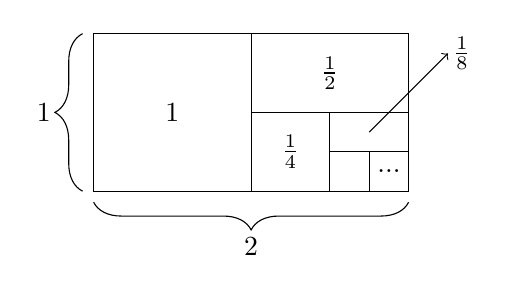
\begin{tikzpicture}[x = 2cm, y = 2cm]
            \draw (0, 0) rectangle ++(2, 1);
            \draw (1, 0) -- (1, 1) node[shift={(-0.5, -0.5)}] {1};
            \draw (1, 0.5) -- (2, 0.5) node[shift={(-0.5, 0.25)}] {$\frac{1}{2}$};
            \draw (1.5, 0) -- (1.5, 0.5) node[shift={(-0.25, -0.25)}] {$\frac{1}{4}$};
            \draw (1.5, 0.25) -- (2, 0.25);
            \draw[->] (1.75, 0.375) -- ++(0.5, 0.5) node[xshift = 5pt] {$\frac{1}{8}$};
            \draw (1.75, 0) -- (1.75, 0.25) node[shift={(0.125, -0.125)}]{...};

            \draw [decorate, decoration= {brace, amplitude = 10pt, raise = 4pt}, yshift = 0]
                (0, 0) -- (0, 1) node[midway, xshift = -18pt] {1};
            
                \draw [decorate, decoration= {brace, mirror, amplitude = 10pt, raise = 4pt}, yshift = 0]
                (0, 0) -- (2, 0) node[midway, yshift = -20pt] {2};
        \end{tikzpicture}

        und $\displaystyle \sum_{k=0}^\infty \frac{1}{2^k} = 2$

        \item \underline{Geometrische Reihe}

        Für $g \in \IR, |q| < 1$ gilt $\displaystyle\sum_{k=0}^\infty q^k = \frac{1}{1-q}$, \\
        denn $\displaystyle S_n = \sum_{k=0}^\infty q^k = \frac{1-q^{n+1}}{1-q}$ (Beweis mit vollständiger Induktion)

        Da $q^{n+1} \xrightarrow[n \to \infty]{} 0$ für $|q| < 1$ (1.10), folgt $S_n \to \dfrac{1}{1-q}$. \\
        Andererseits ist $\displaystyle\sum_{k=0}^\infty q^k$ divergent für $|q| \geq 1$ (2.9)

        \begin{itemize}
            \item In Beispiel d) is $q = \frac{1}{2}$ und $\displaystyle\sum_{k=0}^\infty \frac{1}{2^k} = \frac{1}{1 - \frac{1}{2}} = 2$
            \item $\displaystyle \sum_{k=0}^\infty \qt{-\frac{1}{2}}^k = \frac{1}{1 - \frac{1}{2}} = \frac{2}{3}$

            Diese Reihe ist sogar absolut konvergent.

            \item $\displaystyle \sum_{k=3}^\infty \qt{\frac{2}{3}}^k = \sum_{k=0}^\infty \qt{\frac{2}{3}}^{k+3}
                = \qt{\frac{2}{3}}^3 \cdot \sum_{k=0}^\infty \qt{\frac{2}{3}}^k 
                = \qt{\frac{2}{3}}^3 \cdot \underbrace{\frac{1}{1-\frac{2}{3}}}_{3} = \frac{8}{9}$
            
            \textbf{Achtung bei Index-Verschiebung!} %TODO: Warning symbol?
        \end{itemize}
    \end{enumerate}

    \subsection{Satz: Rechenregeln für Summen}
    Gegeben seien zwei konvergente Reihen mit $\sum_{k=1}^\infty a_k = a, \sum_{k=1}^\infty b_k = b$ \\
    und $c \in \IR$.
    Dann gilt:
    \begin{enumerate}[a)]
        \item $\displaystyle \sum_{k=1}^\infty (a_k + b_k) = \sum_{k=1}^\infty (a_k) + \sum_{k=1}^\infty (b_k) = a + b$
        \item $\displaystyle \sum_{k=1}^\infty c - a_k = c \cdot \sum_{k=1}^\infty a_k = c \cdot a$
        
        Beweis folgt direkt aus 1.13.
    \end{enumerate}
    
    \subsection{Satz: Konvergenz und Divergenzkriterien für Reihen}

    Ist $(S_n)$ mit $S_n = \sum_{k=1}^\infty a_k$ nach oben beschränkt und $a_k > 0 \ \forall k \in \IN$, so ist
    $\sum_{k=1}^\infty a_k$ konvergent. (Folgt direkt aus 1.23)

    \subsection{Cauchy-Kriterium}
    $\sum_{i=1}^\infty a_i$ konvergiert $\eqv \ \forall \epsilon > 0 \ \exists N \in \IN:$
    \[\begin{aligned}
        \underbrace{\abs{a_n + ... + a_k}} < \epsilon \quad \forall k \geq n \geq N \\
        \Big[= \abs{S_k - S_{n - 1}} = \Big|\sum_{i=1}^k a_i - \sum_{i=1}^{n-1} a_i\Big|\Big]
    \end{aligned}\]
    (Folgt aus 1.40)

    \subsection{Satz: Absolute Konvergenz}
    Ist $\sum_{i=1}^\infty a_i$ absolut konvergent, so ist $\sum_{i=1}^\infty$ auch konvergent.

    \textbf{Beweis: } Sei $\epsilon > 0. \imp \ \exists N \in \IN$: $|a_n| + ... + |a_k| < \epsilon \quad \forall k \geq N$.

    Da $|a_n| + ... + |a_k| \leq |a_n| + ... + |a_k| < \epsilon \quad \forall k \geq n \geq N$, \\
    ist 2.6 für $\sum_{i=1}^\infty a_i$ erfüllt.

    \subsection{Korollar: Dreiecksungleichung für Reihen}

    Für jede absolut konvergente Reihe $\sum_{i=1}^\infty a_i$ gilt:
    $$
        \Big| \sum_{i=1}^\infty a_i \Big| \leq \sum_{i=1}^\infty a_i |a_i|
    $$

    \textbf{Beweis: } Sei $\sum_{i=1}^\infty a_i$ absolut konvergent. Dann:
    \[\begin{aligned}
        &\bullet \lim_{k \to \infty}(S_k) \underset{2.1}{=} \lim_{k \to \infty} \qt{\sum_{i=1}^K a_i} \\
        &\text{Da } \lim_{k \to \infty}|S_k| = \Big|\lim_{k \to \infty}\Big| \quad
        \left[\begin{array}{c}
            C_i \to c \\
            \imp |C_i| \to |c|
        \end{array} (1.13) \right], \\
        &\text{ist} \lim_{k \to \infty} \abs{\sum_{i=1}^k a_i} = \abs{\sum_{i=1}^\infty a_i} \ (*) \\
        &\bullet \lim_{k \to \infty} \qt{\sum_{i=1}^k |a_i|} \underset{2.1}{=} \sum_{i=1}^\infty |a_i| \ (**) 
    \end{aligned}\]
    \[\begin{aligned}
        \text{Insgesamt: } &\abs{\sum_{i=1}^k a_i} \leq \sum_{i=1}^k |a_i| \quad \Big| \lim_{k \to \infty} \\
        & \underset{(*),(**)}{\eqv} \abs{\sum_{i=1}^\infty a_i} \leq \sum_{i=1}^\infty |a_i| \quad \qed
    \end{aligned}\]

    \subsection{Satz: Divergenzkriterium}
    Ist $\sum_{i=1}^\infty a_i$ konvergent, so ist $(a_n)$ eine Nullfolge. \\
    D.h. Ist $(a_i)$ keine Nullfolge, so divergiert $\sum_{i=1}^\infty a_i$.

    \textbf{Beweis: } $\sum_{i=1}^\infty a_i$ konvergiert $\underset{2.6}{\imp} \ \forall \epsilon > 0 \ \exists N \in \IN:$

    $|a_n + ... + a_k| < \epsilon \ \forall k \geq n \geq N.$
    
    Wähle $k=1 \imp |a_n| < \epsilon \ \forall n \geq N \imp (a_n)$ Nullfolge. $\qed$

    \subsection{Majorantenkriterium}
    Seien $(a_n), (b_n)$ Folgen in $\IR$ mit $0 \leq a_n \leq b_n \quad \ n \in \IN$. \\
    Ist dann $\sum_{i=1}^\infty b_i$ konvergent, so ist auch $\sum_{i=1}^\infty a_i$ konvergent.

    \textbf{Beweis: } Sei $\epsilon > 0 \underset{2.6}{\imp} \ \exists N \in \IN: |a_n + ... + a_k|$
    
    $\underset{\mathclap{\overbrace{0 \leq a_1 \leq b_i \ \forall i}}}{\leq}|b_n + ... + b_k| < \epsilon \quad \forall k \geq n \geq N \qed$
\ifdefined\MAINDOC\else
\end{document}
\fi
    \ifdefined\MAINDOC\else
\documentclass[10pt, a4paper, fleqn]{article}
\usepackage{base}

\begin{document}
    \title{Skript Mathe 2}
    \date{7. Mai 2018}
    \maketitle
\fi
    \subsection{Bemerkung: Minorantenkriterium}
    Unter den selben Voraussetzungen wie in 2.10 erhält man anhand
    von Kontraposition: Ist $\sum_{i=1}^\infty a_i$ divergent, so ist auch
    $\sum_{i=1}^\infty b_i$ divergent.

    \subsection{Beispiele}
    \begin{enumerate}[a)]
        \item $\displaystyle\sum_{i=1}^\infty \underbrace{\qt{1-\frac{1}{i}}}_{\text{Keine Nullfolge}}$
        ist divergent. (2.9)

        \item $\displaystyle\sum_{i=1}^\infty \frac{1}{\sqrt{i}}$ ist divergent,
        da $0 \leq \frac{1}{i} \leq \frac{1}{\sqrt{i}}$ und 
        $\displaystyle\underbrace{\sum_{i=1}^\infty \frac{1}{i}}_{\mathclap{\text{Harmonische Reihe}}}$ divergent. (2.11)
        
        \item $\displaystyle\sum_{i=1}^\infty \frac{(-1)^i}{2^i}$ ist konvergent,
        weil absolut konvergent. (2.3e, 2.7)

        \item $\displaystyle\sum_{i=0}^\infty \frac{(-1)^i}{i + 1} = 1 - \frac{1}{2} + \frac{1}{3} - \frac{1}{4} \pm ...$
        (alternierende harmonische Reihe) ist konvergent, aber nicht absolut konvergent.
        Die Konvergenz zeigt man mit
    \end{enumerate}

    \subsection{Satz: Leibniz-Kriterium}
    Sei $(a_n)$ monoton fallende Nullfolge reeller Zahlen. Dann ist
    $\sum_{i=0}^{\infty} (-1)^i a_i$ konvergent.
    \textbf{Beweis: }
    Intervallschachtelung (1.26)
    \[
        A_n := \sum_{i=0}^{2n-1} (-1)^i a_i \quad B_n := \sum_{i=0}^{2n} (-1)^i a_i
    \]
    \[\begin{aligned}   
        \bullet \ (A_n)\nearrow : A_{n+1} - A_n &= \sum_{i=0}^{2n+1} (-1)^i a_i -
        \sum_{i=0}^{2n-1} (-1)^n a_i \\
        &= (-1)^{2n+1} a_{2n+1} + (-1)^{2n} a_{2n} \\
        &= a_{2n} - a_{2n+1} \geq 0\text{, da } (a_n) \searrow 
    \end{aligned}\]
    \[\begin{aligned}
        \bullet\text{ Analog: } (B_n)\searrow  
            &\bullet B_n - A_n = a_{2n} \geq 0 \eqv A_n \leq B_n \quad \forall n \in N \\
            &\bullet B_n - A_n = a_{2n} \to 0
    \end{aligned}\]
    $(A_n), (B_n)$ konvergiert mit $\displaystyle \lim_{n \to \infty} A_n = 
    \lim_{n \to \infty} B_n \imp \sum_{i=1}^\infty (-1)^i a_i$ konvergent.

    \subsection{Satz: Wurzelkriterium}
    Sei $(a_n)_{n \geq 1}$ mit $a_n \in \IR$. Dann:
    \begin{itemize}
        \item $\displaystyle \varlimsup_{n \to \infty} \sqrt[n]{|a_n|} < 1 \imp \sum_{k=1}^\infty |a_k|$ konvergent
        \item $\displaystyle \varlimsup_{n \to \infty} \sqrt[n]{|a_n|} > 1 \imp \sum_{k=1}^\infty |a_k|$ divergent
        \item $\displaystyle \varlimsup_{n \to \infty} \sqrt[n]{|a_n|} = 1 \leadsto $ keine allgemeine Aussage für
        $\sum_{k=1}^\infty a_k$ möglich.
    \end{itemize}

    \textbf{Beweis: }

    Sei $\displaystyle \varlimsup_{n \to \infty} \sqrt[n]{|a_n|}$
    \[\begin{aligned}
        \bullet \ a < 1: &\imp \exists \epsilon > 0: a + \epsilon < 1 \\
                         &\imp \exists N \in \IN : \sqrt[n]{|a_n|} \leq a + \epsilon \quad \forall n \geq N, \\
                         &\qquad \text{da } a \text{ größter HP von } \sqrt[n]{|a_n|} \\
                         &\imp |a_n| \leq (a + \epsilon)^n \quad \forall n \geq N \\
                         &\imp \sum_{k=N}^\infty \underbrace{(a + \epsilon)^n}_{<1} \text{ (geometrische Reihe)} \\
                         &\text{ist konvergente Majorante der Reihe } \textstyle{\sum_{k=N}^\infty |a_k|}. \\
                         &\text{Damit konvergiert auch } \sum_{k=1}^\infty |a_k| = \underset{< \infty}{\boxed{\sum_{k=1}^{N-1} |a_k|}} + \sum_{k=1}^\infty |a_n| \\
        \bullet \ a > 1: &\imp \sqrt[n]{|a_n|} > 1 \text{ unendlich oft} \\
                         &\imp |a_n| > 1 \text{ unendlich oft} \\
                         &\imp (a_n) \text{ keine Nullfolge } \underset{2.9}{\imp}
                            \sum_{k=1}^\infty a_k \text{ divergent.} \qed
    \end{aligned}\]

    \subsection{Beispiele}
    \begin{enumerate}[a)]
        \item $\displaystyle \sum_{k=0}^\infty \underset{a_k}{\boxed{\frac{k^3}{3^k}}}$ konvergent, da
        $\displaystyle \varlimsup_{n \to \infty} \frac{\sqrt[n]{n^3}}{\sqrt[n]{3^n}} = 
        \varlimsup_{n \to \infty} \frac{\qt{\sqrt[n]{n}^3}}{3} = \frac{1}{3} < 1$

        \item $\displaystyle \sum_{k=0}^\infty \frac{1}{k^\alpha}$ (allgemeine harminische Reihe) liefert \\
        $\displaystyle \varlimsup_{n \to \infty} \frac{1}{\qt{\sqrt[n]{n}^\alpha}} = 1 \quad (\alpha > 0) \to$ keine Aussage möglich.
    \end{enumerate}

    \subsection{Satz: Quotientenkriterium}
    Sei $(a_n)_{n \geq 1}$ eine Folge in $\IR$ mit $a_n \neq 0 \quad \forall n \in \IN$. Dann:
    \begin{itemize}
        \item $\displaystyle \varlimsup_{n \to \infty} \abs{\frac{a_{n+1}}{a_n}} < 1 \imp \sum_{k=1}^\infty a_k$ absolut konvergent
        \item $\displaystyle \varlimsup_{n \to \infty} \abs{\frac{a_{n+1}}{a_n}} > 1 \imp \sum_{k=1}^\infty a_k$ divergent
        \item $\displaystyle \varlimsup_{n \to \infty} \abs{\frac{a_{n+1}}{a_n}} \geq 1$ und $\displaystyle \varliminf_{n \to \infty} \abs{\frac{a_{n+1}}{a_n}} \leq 1 \leadsto$ keine allgemeine Aussage möglich
    \end{itemize}

    \textbf{Beweis: }
    \[\begin{aligned}
        &\bullet \varlimsup_{n \to \infty} \abs{\frac{a_{n+1}}{a_n}} < a < 1 \quad a \in \IR \\
        &\imp \exists N \in \IN : \abs{\frac{a_{n+1}}{a_n}} \leq a \quad \forall n \geq \IN \\
        &\imp |a_n| \leq a \cdot |a_{n-1}| \leq a^2 \cdot |a_{n-2}| \leq ... \leq a^{n-N} \cdot |a_N| \quad \forall n \geq \IN \\
    \end{aligned}\]
    Da $\displaystyle \sum_{n=N}^\infty a^{n-N} |a_N| = \frac{|a_N|}{a^N} \sum_{n=N}^\infty a^n$ konvergiert (geometrische Reihe), folgt mit 
    
    Majorantenkriterium, dass $\sum_{n=N}^\infty |a_n|$ und somit $\sum_{n=1}^\infty |a_n|$ konvergent ist.
    \[\begin{aligned}
        &\bullet \varlimsup_{n \to \infty} \abs{\frac{a_{n+1}}{a_n}} > 1 \imp \exists N \in \IN : \abs{\frac{a_{n+1}}{a_n}} \geq 1 \quad \forall n \geq N \\
        &\imp |a_n| \geq |a_{n-1}| \geq ... \geq |a_N| > 0 \\
        &\imp (a_n) \text{ keine Nullfolge} \qed
    \end{aligned}\]
    
    \subsection{Beispiele}
    \begin{enumerate}[a)]
        \item $\displaystyle \sum_{k=1}^\infty \frac{2^k}{k!}$ konvergiert, da $\displaystyle \abs{\frac{a_{n+1}}{a_n}} = \frac{2^{\bcancel{n+1}}}{(n+1)\cancel{!}} 
        \cdot \frac{\cancel{n!}}{\bcancel{2^n}} = \frac{2}{n+1} \xrightarrow[n \to \infty]{} 0$ \\
        $\displaystyle \imp \lim_{n \to \infty} \abs{\frac{a_{n+1}}{a_n}} = 0 < 1$

        \item Wie in 2.15b ist für $\displaystyle \sum_{k=1}^\infty \frac{1}{k^\alpha} \quad (\alpha > 0)$ keine Aussage möglich, \\
        da $\displaystyle \abs{\frac{a_{n+1}}{a_n}} = \frac{n^\alpha}{(n+1)^\alpha} = \qt{\frac{n}{n+1}}^\alpha \xrightarrow[n \to \infty]{} 1$

        und somit $\displaystyle \varlimsup_{n \to \infty} \abs{\frac{a_{n+1}}{a_n}} = \varliminf_{n \to \infty} \abs{\frac{a_{n+1}}{a_n}} = 1$
    \end{enumerate}

    \subsection{Bemerkung}
    Mit dem Verdichtungssatz von Cauchy (den wir hier nicht zitieren), kann man zeigen, dass die allgemeine
    harmonische Reihe $\sum_{k=1}^\infty \frac{1}{k^\alpha}$ für $0 < \alpha < 1$ divergiert und für
    $\alpha > 1$ konvergiert.
\ifdefined\MAINDOC\else
\end{document}
\fi
    \ifdefined\MAINDOC\else
\documentclass[10pt, a4paper, fleqn]{article}
\usepackage{base}

\begin{document}
    \title{Skript Mathe 2}
    \date{9. Mai 2018}
    \maketitle

    
\fi
    \subsection{Umordnung von Reihen: Beispiel}
    Man kan Reihen nicht bedenkenlos umordnen:
    \begin{itemize}
        \item $\displaystyle 1 - 1 + \frac{1}{\sqrt{2}} - \frac{1}{\sqrt{2}} + \frac{1}{\sqrt{3}} - \frac{1}{\sqrt{3}} \pm ...$
        \[
            Sn = \begin{cases}
                0 &\text{falls gerade} \\
                \sqrt{\frac{2}{n+1}} &\text{falls n ungerade } \xrightarrow[n \to \infty]{} 0
            \end{cases}
        \]
        \item $\displaystyle 1 + \frac{1}{\sqrt{2}} \underbrace{- 1}_3 + \frac{1}{\sqrt{3}} + \frac{1}{\sqrt{4}} - \underbrace{\frac{1}{\sqrt{2}}}_6 + \frac{1}{\sqrt{5}} + \frac{1}{\sqrt{6}} - \underbrace{\frac{1}{\sqrt{3}}}_9 \pm ...$
        \[
            S_{3n} = \frac{1}{\sqrt{n+1}} + \frac{1}{\sqrt{n+2}} + ... + \frac{1}{\sqrt{2n}} \geq \frac{n}{\sqrt{2n}} = \sqrt{\frac{n}{2}} \xrightarrow[n \to \infty]{} \infty
        \]
    \end{itemize}

    \subsection{Definition: Umordnung}
    $\sum_{k=1}^\infty b_k$ heißt \underline{Umordnung} von $\sum_{k=1}^\infty a_k$, falls \\
    eine bijektive Abbildung $\rho: \IN \to \IN$ existiert mit $b_k = a_{\rho(k)} \quad \forall k \in \IN$

    \subsection{Umordnungssatz}
    Jede Umordnung $\sum_{k=1}^\infty b_k$ einer absolut konvergenten Reihe $\sum_{k=1}^\infty a_k$
    in $\IR$ ist ebenfalls absolut konvergent und es gilt $\sum_{k=1}^\infty b_k = \sum_{k=1}^\infty a_k$ (ohne Beweis)

    \subsection{Riemannscher Umordnungssatz}
    Ist $\sum_{k=1}^\infty a_k$ konvergent, aber nicht absolut konvergent, dann existiert zu jedem $s \in \overline{\IR}$ eine Umordnung
    $\sum_{k=1}^\infty b_k$, mit $\sum_{k=1}^\infty b_k = s$ (ohne Beweis)

    \section{Potenzreihen}
    \subsection{Grundbegriffe und Beispiel}
    \begin{enumerate}[a)]
        \item $P(x) = \sum_{k=0}^\infty x^k$ ist für $|x| < 1$ absolut konvergent (geometrische Reihe), 
        d.h für $x \in \underbrace{(-1, 1)}_{\mathclap{\text{Konvergenzintervall (3.5)}}}$.

        Für $|x| > 1$ ist $P(x)$ divergent.
        \item $P(X) = \sum_{k=0}^\infty k!(x-1)^k$ ist für $x \neq 1$ divergent:

        Quotientenkriterium liefert:
        \[
            \abs{\frac{(x+1)!(x-1)^{k+1}}{k!(x-1)^k}} = (k+1)(x-1) \xrightarrow[k \to \infty]{} \infty \quad \text{für } x \neq 1
        \]
    \end{enumerate}
    \subsection{Definition: Potenzreihen}
    Sei $(a_n)_{n \geq 0}$ reelle Folge und seien $x, x_0 \in \IR.$
    $$P(x) := \sum_{k=0}^\infty a_k (x - x_0)^k$$ 
    heißt Potenzreihe mit Zentrum $x_0$ und Koeffizienten $a_k$

    \subsection{Bemerkung}
    \begin{enumerate}[a)]
        \item In Bsp 3.1a) ist $x_0 = 0$ und $a_k = 1 \ \forall k \in \IN$. \\
        In 3.1b) ist $x_0 = 1$ und $a_k = k!$

        \item In 3.1a) konvergiert $P(x)$ für $x \in (-1, 1)$,
        in 3.1b) lediglich für $x = x_0 = 1$. Es wird sich heraussstellen,
        dass es für eine Potenzreihe $P(x)$ mit Zentrum $x_0$ einen Konvergenzradius
        $\rho \in \overline{\IR}_+ = [0, \infty) \cup \{\infty\}$ gibt (3.5),
        so dass $P(x)$ absolut konvergent für $x \in (x_0 - \rho, x_0 + \rho)$,
        (d.h. $|x-x_0| < \rho$) und divergent für $|x-x_0| > \rho$ ist. (3.7)
    \end{enumerate}

    Dazu zeigt man zunächst:
    \subsection{Satz}
    Sei $P(x) = \sum_{k=0}^\infty a_k(x-x_0)^k$ und $x \in \IR \setminus \{x_o\}$.

    Dann:
    \begin{enumerate}
        \item $P(x_1)$ konvergent $\imp P(x)$ ist absolut konvergent $\forall x \in \IR$ mit \\
        $|x-x_0| < |x_1 - x_0|$
        \item $P(x_1)$ divergent $\imp P(x)$ ist divergent $\forall x \in \IR$ mit \\
        $|x-x_0| > |x_1 - x_0|$ 
    \end{enumerate}
    \textbf{Beweis: }
    \begin{enumerate}
        \item $P(x)$ konvergent $\underset{2.9}{\imp} (a_k(x_1 - x_0)^k)$ Nullfolge
        \[\begin{aligned}
            &\imp \exists K \geq 0: |a_k(x_1 - x_0)| \leq K \forall k \in \IN_0 \\
            &\imp |a_k(x - x_0)^k| = |a_k(x_1 - x_0)^k| \cdot \abs{\frac{x-x_0}{x_1 - x_0}}^k \leq K \cdot \underbrace{\abs{\frac{x-x_0}{x_1 - x_0}}^k}_{\leq 1} \\
            &\underset{2.10}{\imp} P(x) \text{ absolut konvergent für } |x-x_0| < |x_1 - x_0| \text{ (Majorantenkriterium)}
        \end{aligned}\]
        \item Sei $P(x_1)$ divergent und $|x-x_0| > |x_1 - x_0|$. Wäre $P(x)$ konvergent, so wäre
        wegen 1. auch $P(x_1)$ konvergent. \lightning

        Also: $P(x)$ divergent $\qed$
    \end{enumerate}

    \subsection{Definition: Konvergenzradius und Intervall}
    Sei $P(x)$ Potenzreihe mit Zentrum $x_0$. \\
    $$\rho = \sup\{|x-x_0|: P(x) \text{ mit } x \in \IR \text{ konvergent}\} \in [0, \infty) \cup \{\infty\}$$
    heißt \underline{Konvergenzradius} von $P(x)$. 
    
    Für $\rho \in \IR_+$ heißt $(x_0 - \rho, x_0 + \rho)$ \underline{Konvergenzintervall} von $P(x)$. \\
    Ist $\rho = \infty$, so konvergiert $P(x) \ \forall x \in \IR$ (3.7)

    \subsection{Beispiel}
    \begin{enumerate}[a)]
        \item Für $P(x) = \sum_{k=0}^\infty x^k$ ist $\rho = 1$, denn $(-1, 1)$ ist Konvergenzintervall von $P(x), x_0=0$
        \item Für $P(x) = \sum_{k=0}^\infty k!(x-x_0)^k$ ist $\rho = 0$, denn $P(x)$ ist nur für $x=x_0=1$ konvergent.
    \end{enumerate}
    Aus 3.4 ergibt sich direkt 3.7

    \subsection{Korollar}
    Sei $P(X)$ Potenzreihe mit Zentrum $x_0$ und Konvergenzradius $\rho$. 
    
    Dann:
    \begin{enumerate}
        \item $P(X)$ absolut konvergent $\forall x \in \IR$ mit $|x-x_0| < \rho$.
        \item $P(X)$ divergent $\forall x \in \IR$ mit $|x-x_0| > \rho$.
        \item {[Falls $|x-x_0| = \rho \leadsto$ keine allgemeine Aussage möglich]}
    \end{enumerate}
    
\ifdefined\MAINDOC\else
\end{document}
\fi
    \ifdefined\MAINDOC\else
\documentclass[10pt, a4paper, fleqn]{article}
\usepackage{base}

\begin{document}
    \title{Skript Mathe 2}
    \date{14. Mai 2018}
    \maketitle
\fi
    \section*{Berechnung von Konvergenzradien}
    \subsection{Satz: Formel von Cauchy-Hademard}
    
    Sei $(a_k)_{k \geq 0}$ Folge in $\IR$ und $\displaystyle\lambda := \varlimsup_{k \to \infty} \sqrt[k]{|a_k|}$.
    $\rho$ sei der Konvergenzradius von $P(x) = \sum\limits_{k=0}^\infty a_k (x-x_0)^k$.
    
    Dann:
    $$
        \rho = \begin{cases}
            \frac{1}{\lambda} &\text{, falls } \lambda \in \IR > 0 \\
            0 &\text{, falls } \lambda = \infty \\
            \infty &\text{, falls } \lambda = 0
        \end{cases}
    $$

    \textbf{Beweis: }
    Wurzelkriterium: $\displaystyle\lambda := \varlimsup_{k \to \infty} \sqrt[k]{|a_k| \cdot |x-x_0|^k} = \lambda \cdot |x-x_0|$
    \[\begin{aligned}
        &\bullet \underbrace{\lambda \cdot |x-x_0}_{\mathclap{\text{D.h. } P(x) \text{ konvergiert}}} | < 1 \eqv |x-x_0| < \frac{1}{\lambda} \quad (= \rho) \\
        &\bullet \underbrace{\lambda \cdot |x-x_0}_{\mathclap{\text{D.h. } P(x) \text{ divergiert}}} | > 1 \eqv |x-x_0| > \frac{1}{\lambda} \quad (= \rho) \\
        &\imp \rho \text{ Konvergenzradius von } P(x)
    \end{aligned}\]

    \subsection{Beispiel}
    Für welche $x \in \IR$ ist $\sum\limits_{k=1}^\infty \frac{x^k}{k}$ konvergent?
    \[\begin{aligned}
        \bullet &\varlimsup_{k \to \infty} \sqrt[k]{\abs{\frac{1}{k}}} = \varlimsup_{k \to \infty} \frac{1}{\sqrt[k]{k}} = 1 = \lambda \\
        &\underset{3.8}{\imp} \rho = \frac{1}{\lambda} = 1 \\
        &\imp P(x) \text{ konvergent für } x \in \overbrace{(-1, 1)}^{\mathclap{x_0 - \rho, x_0 + \rho}} \text{ und divergiert für } |x| > 1
    \end{aligned}\]
    Untersuche Randwerte für $x = \pm 1$
    \[\begin{aligned}
        &\bullet x=  1: &&P( 1)= \sum_{k=1}^\infty \frac{1}{k} \text{ divergent (harmonische Reihe)} \\
        &\bullet x= -1: &&P(-1)= \sum_{k=1}^\infty \frac{(-1)^k}{k} = \sum_{k=0}^\infty \frac{(-1)^{k+1})}{k+1} \\
            &&&= -\underbrace{\qt{\sum_{k=0}^\infty \frac{(-1)^k}{k+1}}}_{\mathclap{\text{konvergent (2.12d)}}}
    \end{aligned}\]
    $\imp P(-1)$ konvergent

    Insgesamt: $P(x)$ konvergent für $[-1, 1)$, divergent für $|x|>1$ und $x=1$.

    \subsection{Satz: Formel von Euler}
    Sei $(a_k)_{k>0}$ Folge in $\IR, a_k \neq 0 \quad \forall k \in \IN_0$, \\
    $\rho$ Konvergenzradius von $P(x) = \sum\limits_{k=0}^\infty a_k (x-x_0)^k$.
    
    Ist $\qt{\abs{\frac{a_k}{a_{k-1}}}}_{k \geq 0}$ konvergent oder bestimmt gegen $+\infty$ \\
    divergent, so ist $\rho = \lim\limits_{k \to \infty}\abs{\frac{a_k}{a_{k+1}}}$

    \textbf{Beweis: } Wende auf $P(x)$ das Quotientenkriterium 2.16 an. $\qed$

    \subsection{Beispiel: Exponentialfunktion}
    \[\begin{aligned}
        &\sum_{k=0}^\infty \frac{x^k}{k!} \text{ konvergent } \forall x \in \IR: \\
        &\abs{\frac{a_k}{a_{k+1}}} = \frac{1}{k\cancel{!}} \cdot \frac{(k+1)\cancel{!}}{1} = k+1 \xrightarrow[k \to \infty]{} \infty \\
        &\underset{3.10}{\imp} \rho = \infty
    \end{aligned}\]
    Man definiert: $\exp: \IR \to \IR$ mit $\displaystyle \exp(x) = \sum_{k=0}^\infty \frac{x^k}{k!}$ (Exponentialreihe)

    Man kann zeigen:
    \begin{enumerate}
        \item $\exp(x+y) = \exp(x) + \exp(y) \quad \forall x,y \in \IR$ (mit Cauchy-Produkt, hier nicht)
        \item $\exp(x) = e^x, e \approx 2,718$ (Eulersche Zahl)
    \end{enumerate}
    Aus 2.: $\displaystyle  \qquad e = \exp(1) = \sum_{k=0}^\infty \frac{1}{k!} = 1 + 1 + \frac{1}{2!} + \frac{1}{3!} + ...$

    \subsection*{Exkurs: Wie erhält man $\exp(x) = e^x$ ?}
    \begin{enumerate}
        \item Definiere: $\quad e := \lim\limits_{n \to \infty} \qt{1 + \frac{1}{n}}^n$ (1.28)
        \item Zeige: $\quad \exp(1) = e = \lim\limits_{n \to \infty} \qt{1 + \frac{1}{n}}^n$ (später)
        \item Zeige, dass Exponentialgesetze für $\exp(x)$ gelten: 
        
        $\exp(x+y) = \exp(x) + \exp(y) \quad \forall x,y \in \IR$ (hier nicht)
        \item Definiere: $\quad e^x = \exp(x) \quad \forall x \in \IR$
    \end{enumerate}
    
    Dies stimmt dann wegen 3. mit den bekannten Rechenregeln für Potenzen und Wurzen überein:
    \begin{itemize}
        \item $e^n = (\exp(1))^n = \exp(n)$
        \item $\qt{\exp\qt{\frac{n}{m}}}^m = exp(n) = e^n \quad \bigm| \sqrt[n]{\ }$
        
        $\imp \exp\qt{\frac{n}{m}} = (e^n)^{\frac{1}{m}} = e^\frac{n}{m} \quad \forall n,m \in \IN$
    \end{itemize}
    Für irrationale Zahlen wird $e^x$ dann mit Hilfe von $e^x = \exp(x)$ berechnet.
        
    So kann auch ein Computer z.B: $e^\pi$ berechnen, indem $\exp(\pi)$ ermittelt wird.

    \subsection{Bemerkung}
    \begin{enumerate}[a)]
        \item Außer der Funktion $e^x$ gibt es auch andere Funktionen die sich als Reihe
        darstellen lassen, z.B wird in Mathe III gezeigt, dass
        $$\begin{aligned}
            &cos(x) = \sum_{n=0}^\infty (-1)^n \frac{x^{2n}}{(2n)!} \\
            &sin(x) = \sum_{n=0}^\infty (-1)^n \frac{x^{2n + 1}}{(2n + 1)!}
        \end{aligned}$$

        \item Wie Beispiel 3.9 zeigt, ist auf dem Rand des Konvergenzintervalls keine
        allgemeine Aussage über das Konvergenzverhalten der entsprechenden Potenzreihe möglich.
        Für $\rho \neq \infty$ müssen die Randwerte gesondert untersucht werden.
    \end{enumerate}
\ifdefined\MAINDOC\else
\end{document}
\fi
    % Template file
\ifdefined\MAINDOC\else
\documentclass[10pt, a4paper, fleqn]{article}
\usepackage{base}

\begin{document}
    \title{Skript Mathe 2}
    \date{15. Mai 2018} % Date here
    \maketitle
\fi
    \section{Reelle Funktionen}
    \subsection*{Grundbegriffe und Beispiele}
    \subsection{Definition: Abbildung}

    Eine Abbildung $f: A \to B$ besteht aus
    \begin{itemize}
        \item Dem Definitionsbereich $A$ (Menge $A$)
        \item Dem Bildbereich $B$ (Menge $B$)
        \item Einer Zuordnungsvorschrift $f$, die jedem $a \in A$
        \underline{genau} ein Element $b \in B$ zuordnet.
    \end{itemize}
    Man schreibt $b = f(a)$, nennt $b$ Bild/Funktionswert von $a$ und $a$
    (ein) Urbild von $b$.

    Notation: $f: A \to B, a \mapsto f(a)$
    \[\begin{aligned}
        &A&=&\text{ Menge aller Studenten von Mathe II} \\
        &B&=&\text{ \{Raucher, Nichtraucher\}} \\
        &f&=&\text{ Zuordnungsvorschrift, die jedem Studenten zuordnet,} \\
        &&&\text{ ob er/sie raucht/nicht raucht}
    \end{aligned}\]
    
    \subsection{Definition: Reelle Funktion}
    Eine reelle Funktion einer Veränderlichen ist eine \\ 
    Abbildung $f: D \to \IR, D \subseteq \IR$.

    \begin{enumerate}[a)]
        \item $(f \pm g)(x) := f(x) \pm g(x) \quad \forall x \in D$ \\
        Summe/Differenz von $f$ und $g$

        \item $(f \cdot g) := f(x) \cdot g(x) \quad \forall x \in D$ \\
        Produkt von $f$ und $g$

        \item Für $g(x) \neq 0 \quad \forall x \in D$ heißt
        \[
            \qt{\frac{f}{g}}(x) := \frac{f(x)}{g(x)} \quad \forall x \in D
        \]
        Quotient von $f$ und $g$

        \newtikzmark \,
        \item Komposition/Verknüpfung
        \[\begin{aligned}
            &f: D_f \to \IR, g: D_g \to \IR \text{ mit } f(D_f) \subseteq D_g \\
            &f \circ g: D_f \to \IR \\
            &(g \circ f)(x) := g(f(x)) \\
            &\underset{\tikzmark{a}}{D_f} \xrightarrow{f} f(D_f) \subseteq D_g \xrightarrow{g} g(\underset{\tikzmark{b}}{f(D_f)}) \subseteq \IR
        \end{aligned}\]
        \begin{tikzpicture}[remember picture, overlay]
            \draw[->, line width = 1pt] (pic cs:a) to [out = -30, in = -150] node[midway, yshift = -10pt] {$g \circ f$ (``g nach f'')} (pic cs:b);
        \end{tikzpicture}
        \bigskip
    \end{enumerate}
    \subsection{Beispiel}
    \[\begin{aligned}
        &f,g: \IR \to \IR, f(x) = x^2, g(x) = x-1 \\
        &(f+g)(x) = x^2 + x - 1, (f \cdot g)(x) = x^2 (x-1) \\
        &\qt{\frac{f}{g}}(x) = \frac{x^2}{x-1} \text{ für } D = \{x \in \IR | x \neq 1\} \text{ Definitionsbereich von } \frac{f}{g}.\\
        &(f \circ g)(x) = (x-1)^2 \neq \\
        &(g \circ f)(x) = x^2 - 1
    \end{aligned}\]
    \subsection{Definition: Injektiv, Surjektiv, Bijektiv}
    Sei $f: X \to Y$ eine Abbildung. $f$ heißt:
    \begin{enumerate}
        \item Surjektiv $\eqv \ \forall y \in Y \ \exists x \in X: f(x) = y$
        \item Injektiv $\eqv \ (f(x_1) = f(x_2) \imp x_1 = x_2)$
        \item Bijektiv $\eqv f$ ist injektiv und surjektiv 
    \end{enumerate}

    \subsection{Beispiele}
    \begin{enumerate}[a)]
        \item $f: \IR \to \IR, f(x) = x^2$ ist
        \begin{itemize}
            \item nicht surjektiv: z.B gibt es für $y=-1$ kein $x \in \IR$ mit \\
            $f(x) = -1$, da $f(x) = x^2 \geq 0 \quad \forall x \in \IR$
            \item nicht injektiv: $f(-1) = f(1)$ aber $-1 \neq 1$
        \end{itemize}
        \item Jedoch ist $f: \IR_{\geq 0} \to \IR_{\geq 0}$ mit $f(x) = x^2$ bijektiv,
        wie man leicht prüfen kann.
    \end{enumerate}

    \subsection{Definition: Umkehrfunktion, Bild, Urbild}
    Sei $f: X \to Y$ eine Abbildung
    \begin{enumerate}
        \item Für $X_0 \subseteq X$ heißt $f(X_0) := \{f(x) | x \in X_0\}$ Bild von $X_0$
        \item Für $Y_0 \subseteq Y$ heißt $f^{-1}(Y_0) := \{x \in X | f(x) \in Y_0\}$ Urbild von $Y_0$
        \item Ist $f$ bijektiv, so heißt $f^{-1}: Y \to X$ Umkehrfunktion von $f$, \\ 
        falls $f^{-1} \circ f = \id_x$ und $f \circ f^{-1} = \id_y$
    \end{enumerate}

    \subsection{Beispiel}
    \begin{enumerate}[a)]
        \item $f: \IR_{\geq 0} \to \IR_{\geq 0}, f(x) = x^2$ ist bijektiv (4.6b)
        
        Umkehrfunktion: $f^{-1}: \IR_{\geq 0} \to \IR_{\geq 0}, f^{-1}(x) = \sqrt{x}$

        da: $(f \circ f^{-1})(x) = f(f^{-1}(x)) = (\sqrt{x})^2 = \underbrace{x}_{=\id \ \IR_{\geq 0}}$ \\
        $= f^{-1}(f(x)) = \sqrt{x^2} = (f^{-1} \circ f)(x)$

        \underline{Bemerkung:} Die Umkehrfunktion erhält man durch Spiegelung an der Ursprungsgeraden
        \item \underline{Achtung:} Das Urbild existiert immer, auch wenn $f^{-1}$ als Umkehrfunktion nicht existiert.
        
        \underline{Beispiel:} $f: \IR \to \IR, f(x) = x^2 \quad f^{-1}(\{\frac{1}{4}\}) = \{-\frac{1}{2}, +\frac{1}{2}\}$
    \end{enumerate}

    \subsection{Definition: Symmetrie}
    Sei $f(x): \IR \to \IR$ heißt:
    \begin{itemize}
        \item Achsensymmetrisch $\eqv f(x) = f(-x) \quad \forall x \in \IR$ (zur y-Achse)
        \item Punktsymmetrisch $\eqv f(x) = f(-x) \quad \forall x \in \IR$
    \end{itemize}

    \subsection{Definition: Monotonie}
    Sei $f: D \to \IR, D \subseteq \IR$. $f$ heißt (streng) monoton wachsend, \\
    falls $f(x_1) \underset{(<)}{\leq} f(x_2) \quad \forall x_1 \underset{(<)}{\leq} x_2$.

    Falls $f(x_1) \underset{(>)}{\geq} f(x_2) \quad \forall x_1 \underset{(>)}{\geq} x_2$,
    so heißt $f$ (streng) monoton fallend.

    \subsection{Elementare Funktionen}
    \begin{enumerate}[a)]
        \item Konstante Funktion: Sei $c \in \IR \quad f: \IR \to \IR, x \mapsto c$
        \item Identität: $f: \IR \to \IR, x \mapsto x$
        \item Betragsfunktion: $f: \IR \to \IR, x \mapsto |x|$ \\ %TODO: Graph?
            $f$ ist achsensymmetrisch
        \item Monome/Potenzen: 
        $f: \IR \to \IR, x \mapsto x^n \quad (n \in \IN)$
        \begin{itemize}
            \item $n$ gerade: $f$ achsensymmetrisch, weder injektiv noch surjektiv, nicht
            monoton, $f(x) \neq 0 \quad \forall x \in \IR$
            \item $n$ ungerade: $f$ punktsymmetrisch, bijektiv, streng monoton steigend
        \end{itemize}

        \item Wurzenlfunktion
        Sind Umkehrfunktion von Monomen
        \begin{itemize}
            \item $n$ ungerade
            $\imp f(x) = x^n$ bijektiv \\
            $\underset{4.7/3}{\imp}$ Umkehrfunktion existiert und hat die Form
            
            $\sqrt[n]{\ }: \IR \to \IR, x \mapsto \sqrt[n]{x}$
        \end{itemize}
    \end{enumerate}
\ifdefined\MAINDOC\else
\end{document}
\fi
    \ifdefined\MAINDOC\else
\documentclass[10pt, a4paper, fleqn]{article}
\usepackage{base}

\begin{document}
    \title{Skript Mathe 2}
    \date{28. Mai 2018}
    \maketitle
\fi
    \begin{enumerate}[a), start = 6]
        \item[]
        \begin{itemize}
            \item $n$ gerade
            $\imp f: \IR_{\geq 0} \to \IR_{\geq 0}, x \mapsto x^n$ bijektiv

            In diesem Fall hat die Umkehrfunktion die Vorschrift
            \[
                \sqrt[n]{\ }: \IR_{\geq 0} \to \IR_{\geq 0}, x \mapsto \underbrace{\sqrt[n]{x}}_{\geq 0}
            \]
            \textbf{Achtung: } Wenn n gerade, dann hat $x^n = a$ für gegebenes $a \in \IR$
            \begin{itemize}
                \item keine Lösung, falls $a<0$
                \item genaue eine Lösung, falls $a=0$ und zwar $x=0$
                \item genau zwei Lösungen, falls $a>0$ und zwar

                $x_1 = \underbrace{\sqrt[n]{a}}_{> 0} \quad x_2 = \underbrace{-\sqrt[n]{a}}_{< 0}$
            \end{itemize}
        \end{itemize}
        \item Polynome: $p: \IR \to \IR, x \mapsto a_n x^n + a_{n-1} x^{n-1} + ... + a_0 x^0
            = \sum_{k=0}^n a_k x^k$

        $a_0, ..., a_n \in \IR$ heißen Koeffizienten

        Falls $a_n \neq 0$, so heißt $n$ Grad von $p$, man schreibt $\grad(p) = n$

        Für ein Polynom $p$ von Grad $n$ kann man zeigen:
        \begin{enumerate}[1.]
            \item $p$ besitzt höchstens $n$ Nullstellen
            \item Falls $n$ ungerade, ist $p$ surjektiv und besitzt mindestens eine Nullstelle
            \item Falls $n$ gerade, ist $p$ nicht surjektiv und kann daher auch keine Nullstelle haben
        \end{enumerate}
        Bekannte Verfahren zur Berechnung von Nullstellen:
        \begin{itemize}
            \item $\grad(p) = 2$: Mitternachtsformel/pq-Formel
            \item $\grad(p) \geq 3$: Polynomdivision (Mathe III), numerische Verfahren (z.B Newton-Verfahren)
        \end{itemize}
        \item Rationale Funktionen:

        Quotienten von Polyonmen $p,q$ mit $f: D \to \IR$
        \[
            x \mapsto \frac{p(x)}{q(x)} \qquad D=\{x \in \IR \ | \ q(x) \neq 0\}
        \]

        \item Logarithmen und Exponentialfunktion:

        \begin{enumerate}[1.]
            \item der natürliche Logarithmus:

            Man kann zeigen, dass für die Exponentialreihe unter 3.11 gilt:
            \begin{itemize}
                \item $\exp(\IR) = \IR_{> 0}$
                \item $\exp: \IR \to \IR_{> 0}$ ist bijektiv
            \end{itemize}
            Die Umkehrfunktion von $\exp(x)$ ist der natürliche Logarithmus:
            \[
                \ln: \IR_{> 0} \to \IR, x \mapsto \ln(x)
            \]

            \item Exponentialfunktion:

            Sei $q > 0, q \neq 0$. Für $x \in \IQ, x = \frac{a}{b}$ ist
            $q^x = \sqrt[b]{q^a} \quad a \in \IZ, b \in \IN$

            Mit Hilfe der Funktion $\exp(x), \ln(x)$ kann man Exponentialfunktionen
            zu einer beliebigen gegebenen Basis $q$ und $x \in \IR$ definieren:
            \[
                f: \IR \to \IR_{> 0} \quad x \mapsto q^x := \exp(x \cdot \ln(q))     
            \]

            \item Aus 2. ergibt sich die Regel:
            \[
                \ln(q^x) = x \cdot \ln(q) \quad \forall x \in \IR
            \]

            \item Man kann wegen 2. eine Basis $q$ durch eine beliebige andere Basis ausdrücken,
            z.B: $q^x = e^{x \cdot \ln(q)}$ (da $\exp(x) = e^x$ (3.11))

            \item Logarithmus zur Basis $q > 0, q \neq 1$: Bilde die Umkehrfunktion
            von $f(x) = q^x$ (unter 2.)
            \[
                \log_q: \IR_{>0} \to \IR \quad x \mapsto \log_q(x)    
            \]

            \item $log_q$ lässt sich analog zu 4. durch jeden anderen Logarithmus ausdrücken,
            z.B ist 
            \[
                \ln(x) = \ln(q^{\log_q(x)}) \underset{3.}{=} \log_q(x)
                \eqv \log_q(x) = \frac{\ln(x)}{\ln(y)}
            \]

            \item Rechenregeln:
            \begin{itemize}[$-$]
                \item für $f(x) = q^x$ ergeben sich aus 2. und den Regeln für $\exp(x)$ (3.11):
                \begin{itemize}[$\bullet$]
                    \item $q^{x+y} = q^x \cdot q^y \quad \forall x,y \in \IR$
                    \item $q^{-x} = \dfrac{1}{q^x}$, da $1 = q^{x-x} - q^x \cdot q ^{-x} \quad \forall x \in \IR$
                    \item $(q^x)^y = q^{x \cdot y}$
                    \item $(pq)^x = p^x \cdot q^x$
                \end{itemize}
                \item für $\log_q(x)$ ergeben sich aus denen für $q^x$:
                \begin{itemize}[$\bullet$]
                    \item $\log_q(xy) = \log_q(x) + \log_q(y) \quad \forall x,y > 0$
                    
                    denn für $x = q^u, y = q^v$ ist 
                    
                    $\log_q(xy) = \log_q(q^{u+v}) = u + v = \log_q(x) + \log_q(y)$

                    \item $\log_q\qt{\dfrac{q}{x}} = -\log_q(x) \quad \forall x > 0$

                    [mit $q^v = \log_q(x^\alpha) \underset{3./ 6.}{=} \alpha \cdot \log_q(x) \quad \forall x > 0, \alpha \in \IR$]
                \end{itemize}
            \end{itemize}
        \end{enumerate}
        \item Trigonometrische Funktionen:

        \begin{tikzpicture}
            \begin{axis}[
                clip = false,
                width = 0.7\textwidth,
                height = 0.7\textwidth,
                xmin = -1.2, xmax = 1.2,
                ymin = -1.2, ymax = 1.2,
                xtick distance = 1,
                ytick distance = 1,
                axis x line = center,
                axis y line = center,
                axis line style = {->}
            ]
            \coordinate (A) at (0, 0);
            \coordinate (B) at ({sin(45)}, {sin(45)});
            \coordinate (C) at ({cos(45)}, 0);

            \addplot [domain = 0:360, samples = 100] ({cos(x)}, {sin(x))});
            \draw (A) node[dot]{} 
                -- (B) node[dot]{} 
                    node[right, yshift = 5pt] {$P_\varphi = (\cos(\varphi), \sin(\varphi))$}
                -- (C) node[dot]{}
                -- (A);
            \draw pic["$\varphi$", angle radius = 20pt, draw = black] {angle = C--A--B};
            \draw pic["$\cdot$", draw = black] {angle = B--C--A};
            
            % Braces
            \draw[decorate, decoration = {brace, mirror, amplitude = 10pt, raise = 4pt}] 
                (A) -- (C) node[midway, yshift = -20pt] {$\cos(\varphi)$};
            \draw[decorate, decoration = {brace, mirror, amplitude = 10pt, raise = 4pt}]
                (C) -- (B) node[midway, right, xshift = 12pt] {$\sin(\varphi)$};
            
            \end{axis}
        \end{tikzpicture}

        \begin{tabular}{rl}
            $\varphi$: & Winkel zwischen x-Achse und Strecke $\overline{0 \ P_\varphi}$ \\
            $\cos \varphi$: & Ankathete an $\varphi$ in $\Delta(0 \ A_\varphi \ P_\varphi)$ \\
            $\sin \varphi$: & Gegenkathete an  $\varphi$ in $\Delta(0 \ A_\varphi \ P_\varphi)$
        \end{tabular}

        Daraus ergeben sich die Winkelfunktionen:

        \begin{tabular}{rl}
            $\cos:$ & $\IR \to [-1, 1], x \mapsto \cos(x)$ \\
            $\sin:$ & $\IR \to [-1, 1], x \mapsto \sin(x)$ \\
            $\tan:$ & $\IR \setminus \{(k + \frac{1}{2}) \pi \ | \ k \in \IZ\} \to \IR, x \mapsto \dfrac{\sin(x)}{\cos(x)}$ \\
            $\cotan:$ & $\IR \setminus \{k \pi \ | \ k \in \IZ\} \to \IR, x \mapsto \dfrac{\cos(x)}{\sin(x)}$
        \end{tabular}
    \end{enumerate} % Enumerumeritemitemize
\ifdefined\MAINDOC\else
\end{document}
\fi
    \ifdefined\MAINDOC\else
\documentclass[10pt, a4paper, fleqn]{article}
\usepackage{base}

\begin{document}
    \title{Skript Mathe 2}
    \date{30. Mai 2018}
    \maketitle
\fi
    \begin{enumerate}[a), start=9]
        \item[]
        \begin{enumerate}[1.]
            \item Dabei wird der Winkel $\varphi$ meistens im Bogenmaß
            angegeben, d.h. $\varphi \in [0, 2 \pi]$. 
            
            Einige wichtige Werte:

            {\def\arraystretch{1.5}             
            \begin{tabular}{|r|c|c|c|c|c|c|}
                \hline
                Gradmaß: & $0^\circ$ & $30^\circ$ & $45^\circ$ & $60^\circ$ & $90^\circ$ & $180^\circ$ \\
                \hline
                Bogenmaß: & $0$ & $\frac{\pi}{6}$ & $\frac{\pi}{4}$ & $\frac{\pi}{3}$ & $\frac{\pi}{2}$ & $\pi$ \\
                \hline
                $\sin$: & $0$ & $\frac{1}{2}$ & $\frac{1}{\sqrt{2}}$ & $\frac{\sqrt{3}}{2}$ & $1$ & $0$ \\
                \hline
                $\cos$: & $1$ & $\frac{\sqrt{3}}{2}$ & $\frac{1}{\sqrt{2}}$ & $\frac{1}{2}$ & $0$ & $-1$ \\
                \hline
            \end{tabular}}

            Daraus können weitere Werte mit Hilfe des Einheitskreises abgeleitet werden:
            
            \begin{minipage}{0.6\textwidth}
                \begin{tikzpicture}
                    \begin{axis}[
                        clip = false,
                        width = \textwidth,
                        height = \textwidth,
                        xmin = -1.2, xmax = 1.2,
                        ymin = -1.2, ymax = 1.2,
                        xtick distance = 1,
                        ytick distance = 1,
                        axis x line = center,
                        axis y line = center,
                        axis line style = {->}
                    ]
                    \coordinate (A) at (0, 0);
                    \coordinate (B) at ({cos(60)}, {sin(60)});
                    \coordinate (C) at ({cos(60)}, 0);
                    \coordinate (D) at ({cos(120)}, {sin(120)});
                    \coordinate (E) at ({cos(120)}, 0);
        
                    \addplot [domain = 0:360, samples = 100] ({cos(x)}, {sin(x))});
                    \draw (A) -- (B) -- (C) -- (A);
                    \draw (A) -- (D) -- (E) -- (A);
                    
                    \draw pic["$\frac{\pi}{3}$", angle radius = 18pt, draw = black] {angle = C--A--B};
                    \draw pic[angle radius = 23pt, draw = black] {angle = C--A--D};
                    \draw [->] (-0.8, 1) node[left] {$\frac{2\pi}{3}$} -- (-0.05, 0.2);

                    % Braces
                    \draw[decorate, decoration = {brace, mirror, amplitude = 5pt, raise = 2pt}] 
                        (A) -- (C) node[midway, yshift = -15pt] {$\frac{1}{2}$};
                    \draw[decorate, decoration = {brace, mirror, amplitude = 5pt, raise = 2pt}] 
                        (E) -- (A) node[midway, yshift = -15pt] {$-\frac{1}{2}$};
                    \draw[decorate, decoration = {brace, mirror, amplitude = 5pt, raise = 2pt}]
                        (C) -- (B) node[midway, right, xshift = 5pt] {$\frac{\sqrt{3}}{3}$};
                    
                    \end{axis}
                \end{tikzpicture}
            \end{minipage}
            \begin{minipage}{0.4\textwidth}
                \[\begin{aligned}
                    &\cos\qt{\frac{2\pi}{3}} = -\frac{1}{2} = -\cos\qt{\frac{\pi}{3}} \\
                    &\sin\qt{\frac{2\pi}{3}} = \frac{\sqrt{3}}{2} = -\sin\qt{\frac{\pi}{3}} \\
                \end{aligned}\]
            \end{minipage}
            \item $\sin$ und $\cos$ sind nicht bijektiv. Jedoch ist
            $\sin [-\frac{\pi}{2}, \frac{\pi}{2}] \to [-1, 1]$ und $\cos [0, \pi] \to [-1, 1]$ bijektiv.
            Die Umkehrfunktionen sind:

            \begin{tabular}{rl}
                $\arcsin$: & $[-1, 1] \to [-\frac{\pi}{2}, \frac{\pi}{2}]$ \\
                $\arccos$: & $[-1, 1] \to [0, \pi]$
            \end{tabular}

            Entsprechend erhält man:

            \begin{tabular}{rl}
                $\arctan$: & $\IR \to (-\frac{\pi}{2}, \frac{\pi}{2})$ \\
                $\arccotan$: & $\IR \to (0, \pi)$
            \end{tabular}

            \item
            \begin{itemize}
                \item Es ist $\sin(x + \frac{\pi}{2}) = \cos(x) \quad \forall x \in \IR$
                \item $\sin, \cos$ sind $2\pi$-periodisch, d.h. \\
                $\sin(x + 2 \pi) = \sin(x), \cos(x + 2 \pi) = \cos(x)$
                \item $\tan, \cotan$ sind $\pi$-periodisch
            \end{itemize}

            \item Symmetrien
            \[\begin{aligned}
                \cos(x) &= \cos(-x) & \forall x \in \IR \\
                \sin(x) &= -\sin(-x) & \forall x \in \IR \\
                \tan(x) &= -\tan(-x) &\forall x \in \IR \\
                \cotan(x) &= -\cotan(-x) & \forall x \in \IR
            \end{aligned}\]

            \item Rechenregeln
            \begin{enumerate}[a)]
                \item $\sin x + \cos x = 1 \quad \forall x \in \IR$
                \item Additionstheoreme
                \begin{itemize}
                    \item $\sin(x+y) = \sin(x) \cdot \cos(y) + \cos(x) \cdot \sin(y)$
                    \item $\cos(x+y) = \cos(x) \cdot \cos(y) - \sin(x) \cdot \sin(y)$
                \end{itemize}
            \end{enumerate}
        \end{enumerate}
    \end{enumerate}

    \section{Grenzwerte von Funktionen und Stetigkeit}
    \subsection{Definition: Grundbegriffe und Beispiele}

    Sei $M \subseteq \IR$.
    \begin{enumerate}[a)]
        \item $X_0 \in \IR$ heißt Häufungspunkt von $M$ \\
         $:\eqv$ Es gibt eie Folge $(X_n)$ in
        $M \setminus \{X_0\}$ mit $X_n \mapsto X_0$
        
        \item $X_0 \in M$ heißt isolierter Punkt von $M$ \\
        $:\eqv X_0$ ist kein Häufungspunkt von M
    \end{enumerate}

    \subsection{Beispiele}
    \begin{enumerate}[a)]
        \item $M = (0, 1) \cup \{2\} \cup (3, 4)$
        \begin{itemize}
            \item Menge der Häufungspunkte von $M$: \\
            $H = [0,1] \cup [3,4]$
            denn z.B für $X_0 = \frac{1}{2}$ hat die Folge
            $(\frac{1}{2} - \frac{1}{n})_{n \geq 3}$ den Limes
            $X_0$ und liegt in $M \setminus \{X_0\}$.

            Auf analoge Weise können für jedes andere $X_0 \in M$ \\
            Folgen in $M \setminus \{X_0\}$ konstruiert werden.

            \item Einziger isolierter Punkt in $M$ ist $2$, denn es gibt in \\ 
            $M \setminus \{2\} = (0,1) \cup (3,4)$ keine Folge
            mit Grenzwert $2$.
        \end{itemize}
        \item $M = \{\frac{1}{n} \ | \ n \in \IN\}$
        \begin{itemize}
            \item Menge der HP von $M$: $\{0\}$
            \item Menge der isolierten Punkte: $M$
        \end{itemize}
    \end{enumerate}

    \subsection{Bemerkung}
    Ein isolierter Punkt $X_0$ von $M$ liegt vor, wenn es ein $\epsilon > 0$ gibt,
    so dass \\ $|X - X_0| \geq \epsilon \quad \forall x \in M \setminus \{X_0\}$,
    z.B ist in 5.2a $|X - 2| \geq 1 \quad \forall x \in M \setminus \{2\}$

    \subsection{Definition Grenzwert I}
    Sei $f: D \to \IR$ reelle Funktion und $a \in \IR$.
    Ist $X_0$ ein Häufungspunkt von $D$, so sagt man $f$ hat in $X_0$ den Grenzwert
    $a$, oder $f(x)$ konvergiert gegen $a$ für $x \to a :\eqv \lim\limits_{n \to \infty} f(X_n) = a$,
    für jede beliebige Folge $(X_n)$ in $D \setminus \{X_0\}$ mit $X_n \to X_0$.

    Schreibweise: $\lim\limits_{x \to X_0} f(x) = a$ oder
    $f(x) \to a$ für $x \to X_0$

    \subsection{Beispiele}
    \begin{enumerate}[a)]
        \item $f: \IR \to \IR, x \mapsto x^2, X_0 = 1$

        Für $(X_n)$ in $\IR \setminus \{1\}$ mit $X_n \to 1$ ist
        $f(X_n) = {X_n}^2 \xrightarrow[n \to \infty]{} 1$ (1.13/3)

        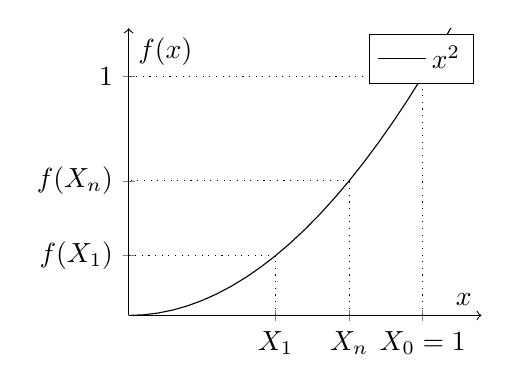
\begin{tikzpicture}[
                declare function = {f(\x) = \x^2;}
            ]
            \begin{axis}[
                width = 0.5\textwidth,
                xlabel = {$x$},
                ylabel = {$f(x)$},
                xmin = 0, ymin = 0,
                xmax = 1.2, ymax = 1.2,
                axis x line = center,
                axis y line = center,
                axis line style = {->},
                xtick = {0.5, 0.75, 1},
                xticklabels = {$X_1$, $X_n$, $X_0 = 1$},
                ytick = {0.25, 0.5625, 1},
                yticklabels = {$f(X_1)$, $f(X_n)$, $1$},
                domain = 0:1.2
            ]
            \draw[dotted] (0.5, 0) -- (0.5, {f(0.5)}) -- (0, {f(0.5)});
            \draw[dotted] (0.75, 0) -- (0.75, {f(0.75)}) -- (0, {f(0.75)});
            \draw[dotted] (1, 0) -- (1, 1) -- (0, 1);

            \addplot[color = black] {f(x)};
            \legend{$x^2$}
            \end{axis}
        \end{tikzpicture}

        \item Es muss für jede Folge $(X_n)$ in $D \setminus \{X_0\}$ mit $X_n \to X_0$ gelten:
        $f(X_n) \to a$

        Gegenbeispiel: $f: \IR \to \IR \quad f(x) = \begin{cases}
            -1 & x < 0 \\
            +1 & x > 0
        \end{cases}$

        \begin{tikzpicture}[
            declare function = {f(\x) = \x^2;}
        ]
        \begin{axis}[
            width = 0.6\textwidth,
            height = 0.3\textwidth,
            xlabel = {$x$},
            ymin = -1.2, ymax = 1.2,
            xmin = -1, xmax = 1,
            xtick = \empty,
            axis x line = center,
            axis y line = center,
            axis line style = {->},
            samples at = {-1, -0.001, 0, 0.001, 1}
        ]
        \addplot[color = black] {sign(x)};  
        \end{axis}
    \end{tikzpicture}

    Grenzwert in $X_0 = 0$ existiert nicht, denn \\
    $f(-\frac{1}{n}) = -1 \xrightarrow[n \to \infty]{} -1$ und \\
    $f(\frac{1}{n}) = 1 \xrightarrow[n \to \infty]{} 1$, obwohl 
    $\frac{-1}{n} \to X_0$ und $\frac{1}{n} \to X_0$
    \end{enumerate}

    \subsection{$\epsilon$--$\varphi$--Kriterium}
    Sei $f: D \to \IR$ reelle Funktion, $X_0$ HP in $D$,
    $a \in \IR$. Dann:
    \[\begin{aligned}
        \lim_{x \to X_0} f(x) = a \eqv \forall \epsilon > 0 \ \forall x \in D \setminus \{X_0\}: \\
        \underbrace{|x-X_0| < \delta \imp |f(x) - a| < \epsilon}_{(*)}
    \end{aligned}\]

\iffalse %TODO Figure out what the graph for this is
    \textbf{Anschaulich:}

    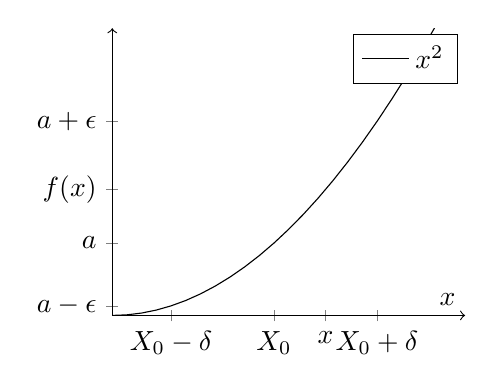
\begin{tikzpicture}[
        declare function = {f(\x) = \x^2;}
    ]
        \begin{axis}[
            width = 0.5\textwidth,
            xlabel = {$x$},
            xmin = 0, ymin = 0,
            xmax = 1.2, ymax = 1.2,
            axis x line = center,
            axis y line = center,
            axis line style = {->},
            xtick = {0.2, 0.55, 0.725, 0.9},
            xticklabels = {$X_0 - \delta$, $X_0$, $x$, $X_0 + \delta$},
            ytick = {0.04, 0.3025, 0.525625, 0.81},
            yticklabels = {$a - \epsilon$, $a$, $f(x)$, $a + \epsilon$},
            domain = 0:1.2
        ]
        \addplot[color = black] {f(x)};
        \legend{$x^2$}
        \end{axis}

    \end{tikzpicture}
\fi
\ifdefined\MAINDOC\else
\end{document}
\fi
    \ifdefined\MAINDOC\else
\documentclass[10pt, a4paper, fleqn]{article}
\usepackage{base}

\begin{document}
    \title{Skript Mathe 2}
    \date{4. Juni 2018}
    \maketitle
\fi

Existenz von $a$ bedeutet: Wenn $x$ nahe genug bei $X_0$ ist, so ist auch $f(x)$ sehr
nahe an $a$.

\textbf{Beweis: } %TODO: Formatting

$(\Leftarrow):$ Gelte (*). Sei $(X_n)$ in $D \setminus \{X_0\}, X_n \to X_0.$
Z.z.: $f(X_n) \to a$

Da $X_n \to X_0$, gibt es $N \in \IN$ mit $|X_n - X_0| < \delta \quad \forall n \geq N$ (1.5) \\
$(*) \imp |f(X_n) - a| < \epsilon \quad \forall n \geq N$ \\
$\underset{1.5}{\imp} f(X_n) \xrightarrow[n \to \infty]{} q$

$(\Rightarrow):$ Mit Kontraposition: Gelte (*) nicht. \\
$\imp \exists \epsilon > 0$ derart, dass für jedes $n \in \IN$ ein $X_n \in D \setminus \{X_0\}$
existiert mit \\
$|X_n - X_0| < \delta$ und $|f(X_n) - a| \geq \epsilon$. \\
$\underset{1.5}{\imp} f(X_n) \ \cancel{\to} \ n$ für $X_n \to X_0. \qed$

\subsection{Beispiel}
$f: \IR \to \IR, f(x) = ax + b$ mit $a, b \in \IR$. Es ist $\lim\limits_{x \to X_0} f(x) = f(X_0).$

Prüfe mit $\epsilon$--$\delta$--Kriterium:

Sei $\epsilon > 0$. Für $\delta = \dfrac{\epsilon}{|a|}$ ist \\
$|f(x) - f(X_0)| = ax + b - aX_0 - b = |a| \cdot \underbrace{|x - X_0|}_{< \delta} < |a| \cdot \dfrac{\epsilon}{|a|} = \epsilon$

\subsection{Definition: Grenzwert II}
Sei $X_0$ HP von $D \subseteq \IR$ und $f: D \to \IR$.
\begin{enumerate}[1.]
    \item $f$ hat in $X_0$ den Grenzwert $+\infty \ (-\infty) :\eqv f(X_n) \to +\infty (-\infty)$ für
    jede Folge $(X_n)$ in $D \setminus \{X_0\}$ mit $X_n \to X_0$.

    Schreibweise: $\lim\limits_{x \to X_0} f(x) = +\infty \ (-\infty)$

    \item Ist $\sup D = \infty \ (\inf D = -\infty)$, so hat $f(x)$ \\
    Limes $a \in \IR$ für $x \to \infty \ (x \to -\infty) :\eqv f(X_n) \to a$ für jede Folge
    in $D$ mit $X_n \to \infty \ (X_n \to -\infty)$
\end{enumerate}

\subsection{Beispiele}
\begin{enumerate}[a)]
    \item $f: \IR \setminus \{0\} \to \IR, f(x) = \dfrac{1}{x^2}$
    \begin{enumerate}[1.]
        \item $\displaystyle \lim_{x \to 0} \frac{1}{x^2} = \infty$, da für jede Nullfolge $(X_n)$ \\
        in $\IR \setminus \{0\}$ gilt: $\dfrac{1}{\underbrace{{X_n}^2}_{=0}} \xrightarrow[n \to 0]{} + \infty$
        \item $\displaystyle \lim_{x \to \infty} \frac{1}{x^2} = 0$, da für jedes $(X_n)$ \\
        in $\IR$ mit $X_n \to \infty: \dfrac{1}{{X_n}^2} \xrightarrow[n \to \infty]{} 0$
    \end{enumerate}

    \item Es gilt für jedes $m \in \IN_0$:
    \begin{enumerate}[1.]
        \item $\displaystyle \lim_{x \to \infty} \frac{\exp(x)}{x^m} = \infty$
        \item $\displaystyle \lim_{x \to -\infty} x \cdot \exp(x) = 0$
    \end{enumerate}
    \textbf{Beweis: }
    \begin{enumerate}[1.]
        \item $\displaystyle
            \exp(x) = \sum_{k = 0}^\infty \frac{x^k}{k!} \geq \frac{X^{m+1}}{(k+1)!} \quad \forall x \geq 0
        $ \\ $\displaystyle 
            \imp \frac{\exp(x)}{x^m} \geq \frac{x^{\cancel{m} + 1}}{(k+1)x^{\cancel{m}}} = \frac{x}{(k+1)!} \to \infty
        $ \\
        für $x \to \infty$
        \item $\displaystyle
            x^m \cdot \exp(x) = \frac{(-1)^m (-x)^m}{\exp(-x)} = (-1)^m \cdot \frac{1}{\boxed{\frac{\exp(-x)}{(-x)^m}} \underset{1.}{\to} \infty}
        $ \\
        für $x \to -\infty$
    \end{enumerate}
\end{enumerate}

\subsection{Definition: Rechts--/Linksseitiger Grenzwert}
\begin{enumerate}[1.]
    \item Ist $X_0$ HP von $D \cap (X_0, \infty)$, so hat $f$ in $X_0$ den rechtsseitigen Grenzwert
    $a \in \IR :\eqv f(X_n) \to a$ für jede Folge $(X_n)$ in $D \cap (X_0, \infty)$ mit $X_n \to X_0$.

    Schreibweise: $\lim\limits_{x \to {X_0}^+} f(x) = a$

    \item Ist $X_0$ HP von $D \cap (-\infty, X_0)$, so hat $f$ in $X_0$ den linksseitigen Grenzwert
    $a \in \IR :\eqv f(X_n) \to a$ für jede Folge $(X_n)$ in $D \cap (-\infty, X_0)$ mit $X_n \to X_0$.

    Schreibweise: $\lim\limits_{x \to {X_0}^-} f(x) = a$
\end{enumerate}

\subsection{Beispiel}
$f: \IR \to \IR \quad x \mapsto \begin{cases}
    -1 & x < 0 \\
    1 & x \geq 0
\end{cases}$

\begin{itemize}
    \item $\lim\limits_{x \to 0^+} f(x) = 1$, da $f(X_n) = 1 \to 1$ \\
    für $(X_n)$ in $(0, \infty)$ und $(X_n) \to 0$

    \item $\lim\limits_{x \to 0^-} f(x) = -1$, da $f(X_n) = -1 \to -1$ \\
    für $(X_n)$ in $(-\infty, 0)$ und $(X_n) \to 0$
\end{itemize}

\subsection{Bemerkung}
Aus 5.11 ist ersichtlich: Der Grenzwert einer Funktion $f$ in $X_0$ existiert $\eqv$ Der Links--
und Rechtsseitige Grenzwert von $f$ in $X_0$ existieren und übereinstimmen.

\subsection{Beispiele}
\begin{enumerate}[a)]
    \item $\lim_{x \to 0} \frac{1}{|x|} = \infty$, aber $\lim_{x \to 0} \frac{1}{x}$ existiert nicht, \\
    da $\lim_{x \to 0^+} \frac{1}{x} = +\infty \neq \lim_{x \to 0^-} \frac{1}{x} = - \infty$

    \item $\lim_{x \to \infty} x = \infty$, $\lim_{x \to -\infty} x = -\infty$
\end{enumerate}

\subsection{Definition: Stetigkeit}
Sei $f: D \to \IR, D \subseteq \IR$
\begin{enumerate}[a)]
    \item f heißt stetig in $X_0 \in D$, falls
    \[
        \underbrace{\lim_{x \to X_0} f(x)}_A \underbrace{= f(X_0)}_B    
    \]
    \item $f$ heißt stetig, falls $f$ in jedem Punkt $X_0 \in D$ stetig ist.
\end{enumerate}

\subsection{Bemerkung}
\begin{enumerate}[a)]
    \item In 5.15a prüft man zwei Bedingungen: A) Der Grenzwert von $f$ in $X_0$ existiert und 
    B) ist gleich $f(X_0)$.

    \item Wegen 5.6 ist $f$ in $X_0 \in D$ stetigt $\eqv$
    \[
        \forall \epsilon > 0 \ \exists \delta > 0 \ \forall x \in D: |x-X_0| < \delta
        \imp |f(x) - f(X_0)| < \epsilon    
    \]
\end{enumerate}

\subsection{Beispiele}
\begin{enumerate}[a)] 
    \item $f: \IR \to \IR, f(x) = x^2$ ist in jedem $X_0 \in D$ stetig:

    $\lim\limits_{x \to X_0} f(x) = f(X_0)$, da für $(X_n)$ in $D \setminus \{X_0\}$ gilt:
    \[
        \underbrace{f(X_n) = X_n^2 \to {X_n}^2 \to {X_0}^2}_{A} \underbrace{= f(x)}_{B}    
    \]
    \item Wegen 5.4 ist $f: \IR \to \IR$ mit $f(x) = ax + b$ stetig.
\end{enumerate}

\subsection{Satz}
Sei $f: D \to \IR, D \subseteq \IR$.

Gibt es ein k > 0 mit $|f(x) - f(X_0)| \leq k \cdot |x - X_0| \quad \forall x \in D$, \\
so ist $f$ stetig in $X_0$.

\textbf{Beweis: }
Sei $\epsilon > 0$. Wähle $\delta = \dfrac{\epsilon}{\delta}$
\[
    \imp |f(x) - f(X_0)| \leq k \cdot |\underbrace{x - X_0}_{< \delta}| < k \cdot \delta = \epsilon \qed   
\]

\ifdefined\MAINDOC\else
\end{document}
\fi
    \ifdefined\MAINDOC\else
\documentclass[10pt, a4paper, fleqn]{article}
\usepackage{base}

\begin{document}
    \title{Skript Mathe 2}
    \date{06. Juni 2018} % Date here
    \maketitle
\fi

\subsection{Bemerkung}
Wähle $\delta = \dfrac{\epsilon}{k}$
\[
    \imp |f(x) - f(X_0)| \leq k \cdot |\underbrace{x - X_0}_{< \delta}| < k \cdot \delta = \epsilon \qed    
\]

\subsection{Beispiel}
\begin{enumerate}[a)]
    \item Anschauung zu 5.14a

    Es gibt 4 Fälle:

    \pgfplotsset{
        compat = 1.15,
        example axis/.style = {
            width = \textwidth,
            ytick = \empty, xtick = {10},
            xticklabels = {$X_0$},
            yticklabels = {$f(X_0)$},
            xmin = 0, xmax = 15,
            ymin = 0, ymax = 35,
            axis x line = center,
            axis y line = center,
            axis line style = {->},
            domain = 0:15
        },
        /pgf/declare function = {
            f141(\x) = -8.60*10^(-3)*x^4 
                +2.99*10^(-1)*x^3 
                -3.40*x^2 
                +12.61*x 
                +10;
        }
    }

    \begin{minipage}{0.4\textwidth}
        \begin{flushright}
            \begin{tikzpicture}
                \begin{axis}[
                    example axis,
                    ytick = {9}
                ]
                \draw[dashed] (10, 0) -- (10, 9) -- (0, 9);
                \addplot[color = black] {f141(x)};
                \draw (10, 9) node[circle, fill = black, scale = 0.3]{};
                \end{axis}
            \end{tikzpicture}
        \end{flushright}
    \end{minipage}
    \hfill
    \begin{minipage}{0.5\textwidth}
        $\lim\limits_{x \to X_0} f(x)$ existiert \\
        und ist gleich $f(x)$
    \end{minipage}

    \begin{minipage}{0.4\textwidth}
        \begin{flushright}
            \begin{tikzpicture}[
                declare function = {
                    g(\x) = f141(x) + 10;
                }
            ]
                \begin{axis}[example axis]
                \draw[dashed] (10, 0) -- (10, 19);
                \addplot[color = black, domain = 0:10] {f141(x)};
                \addplot[color = black, domain = 10:15] {g(x)};
                \end{axis}
            \end{tikzpicture}
        \end{flushright}
    \end{minipage}
    \hfill
    \begin{minipage}{0.5\textwidth}
        $\lim\limits_{x \to X_0} f(x)$ existiert nicht
    \end{minipage}

    \begin{minipage}{0.4\textwidth}
        \begin{flushright}
            \begin{tikzpicture}
                \begin{axis}[example axis, ytick = {27}]
                \draw[dashed] (10, 0) -- (10, 27) -- (0, 27);
                \addplot[color = black] {f141(x)};  
                \draw (10, 9) node[circle, draw = black, fill = white, scale = 0.5]{};
                \draw (10, 27) node[circle, fill = black, scale = 0.3]{};
                \end{axis}
            \end{tikzpicture}
        \end{flushright}
    \end{minipage}
    \hfill
    \begin{minipage}{0.5\textwidth}
        $\lim\limits_{x \to X_0} f(x)$ existiert \\
        und ist ungleich $f(X_0)$
    \end{minipage}

    \item Schule: $f$ ist stetig, wenn man $f$ ``ohne Absetzen'' zeichnen kann.

    Gegenbeispiel: $f:\IR \setminus \{0\} \to \IR, f(x) = \dfrac{1}{x}$ stetig
    auf $\IR \setminus \{0\}$

    \item Dirichlet--Funktion:
    \[f: \IR \to \IR, f(x) = \begin{cases}
        1 & x \in \IR \\
        0 & x \in \IR \setminus \IQ
    \end{cases}\]
    unstetig in jedem $X_0 \in \IR$.

    Mit $\epsilon$--$\delta$--Kriterium:

    Sei $\delta > 0$.
    \begin{enumerate}[1.]
        \item $X_0 \in \IQ \imp \ \exists x \in \IR \setminus \IQ: |x-X_0| < \delta$
        \item $X_0 \in \IR \setminus \IQ \imp \ \exists x \in \IR: |x-X_0| < \delta$
    \end{enumerate}
\end{enumerate}

\section*{Eigenschaften stetiger Funktionen}
\subsection{Satz: Rechenregeln für stetige Funktionen}

\begin{enumerate}[a)]
    \item Seien $f, g: D \to \IR$ stetig in $X_0 \in D, D \subseteq \IR, c \in \IR$. \\
    Dann sind auch $c \cdot f, f \pm g, f \cdot g$ und $ \dfrac{f}{g}$ 
    (für $g(x) \neq 0 \ \forall x \in D$) stetig.

    \item Seien $D, D' \subseteq \IR, f: D \to IR, g: D' \to \IR, f(D) \subseteq D'$. \\
    $f, g$ stetig $\imp g \circ f$ stetig.
\end{enumerate}

\textbf{Beweis: }
\begin{enumerate}[a)]
    \item Folgt direkt aus 5.14
    \item Mit 1.14 $\qed$
\end{enumerate}

\subsection{Bemerkung}
Wegen 5.16b und 5.20
\begin{enumerate}[a)]
    \item sind Monome und Polynome stetig
    \item Wegen a und 5.20a sind rationale Funktionen stetig
    \item Potenzreihen sind auf ihrem Konvergenzintervall stetig (zeigen wir hier nicht).
    Daher sind $\exp, \sin, \cos, \tan, \cotan$ (vgl. 3.11, 3.12) auch stetig.
\end{enumerate}

\subsection{Beispiele und Bemerkung zu Definitionslücken}
\begin{enumerate}[a)]
    \item Hebbare Definitionslücke:

    Sei $f: D \to \IR$ und $X_0$ HP von $X_0 \notin D$.
    Ist $\lim\limits_{x \to X_0} f(x) = a$, so heißt $X_0$
    stetig hebbare Definitionslücke von $f$.
    \[f: D \cup \{X_0\} \to \IR \quad \tilde{f}(x) = \begin{cases}
        f(x) & x \in D \\
        a & x = X_0
    \end{cases}\]
    heißt Fortsetzung von $f$ auf $D \cup \{X_0\}$.

    Beispiel: $f: \IR \setminus \{1\} \to \IR \quad f(x) = \dfrac{x^2 - 1}{x - 1}$
    \[
        \lim_{x \to 1} f(x) = \lim_{x \to 1} \frac{(x-1) \cdot (x+1)}{(x-1)} = 2    
    \]
    % TODO Graph?
    \[
        \tilde{f}: \IR \to \IR \quad \tilde{f}(x) = \begin{cases}
            f(x) & x \neq 1 \\
            2 & x = 1
        \end{cases} = x + 1
    \]

    \item Polstelle:

    Gilt für die Nullstelle $X_0$ des Nenners einer rationalen Funktion, dass
    $f(x) \to \pm \infty$, für $x \to X_0^-$ oder $x \to X_0^+$, so heißt $X_0$
    Polstelle.

    Beispiel: $f(x) = \dfrac{1}{x}$ hat Polstelle bei $X_0 = 0$.

    \item $f: \IR \setminus \{0\} \to \IR, f(x) = \sin\qt{\dfrac{1}{x}}$ hat in $X_0 = 0$ keinen Grenzwert.
 
    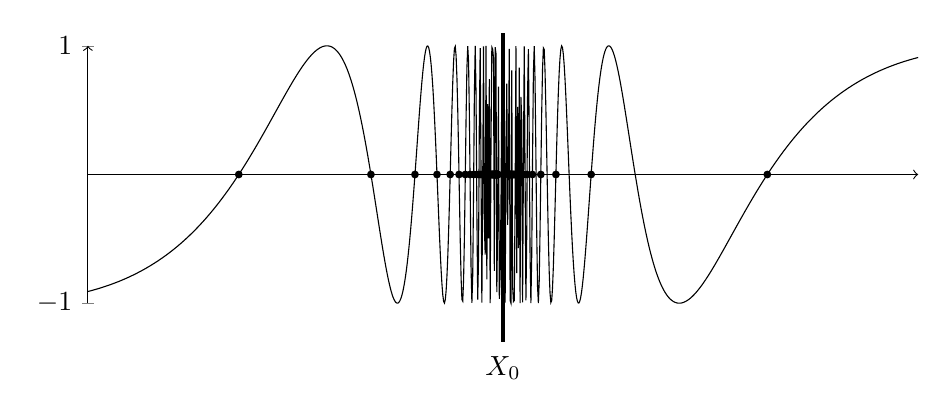
\begin{tikzpicture}
        \begin{axis}[
            width = \textwidth,
            height = 0.4\textwidth,
            xtick = {0}, ytick = {-1, 1},
            xticklabels = {$X_0$},
            ymin = -1, ymax = 1,
            axis x line = center,
            axis y line = left,
            axis line style = {->},
            domain = -0.5:0.5,
            xticklabel style = {yshift = -60pt},
            clip = false
        ]
         
        \foreach \k in {-1,...,-50,1,...,50} {
            \edef\tmp{\noexpand\draw ({1/(\k*pi)}, 0) node[circle, fill = black, scale = 0.3] {};}
            \tmp
        }
        \addplot[color = black, samples = 1000] {sin(deg(1/x))};
        \draw[line width = 0.5mm] (0, -1.3) -- (0, 1.1);
        \end{axis}

    \end{tikzpicture}

    Man nennt $X_0$ Oszillationsstelle:
    \begin{itemize}
        \item $X_n = \dfrac{1}{n \pi} \to 0$ und $f(X_n) = \sin(n \pi) = 0$
        \item $Y_n = \dfrac{1}{n \cdot 2 \pi + \frac{\pi}{2}} \to 0$ und $f(Y_n) = \sin(2 \pi n + \frac{\pi}{2}) = 1$
    \end{itemize}
    \[\begin{aligned}
        &\imp f(Y_n) \to 1 \\
        &\imp \lim_{x \to 0} f(x) \text{ existiert nicht.}
    \end{aligned}\]

    \item $f: \IR \setminus \{0\} \to \IR \quad f(x) = x \cdot \sin\qt{\dfrac{1}{x}}$
    hat in $X_0 = 0$ \\ 
    eine hebbare Definitionslücke

    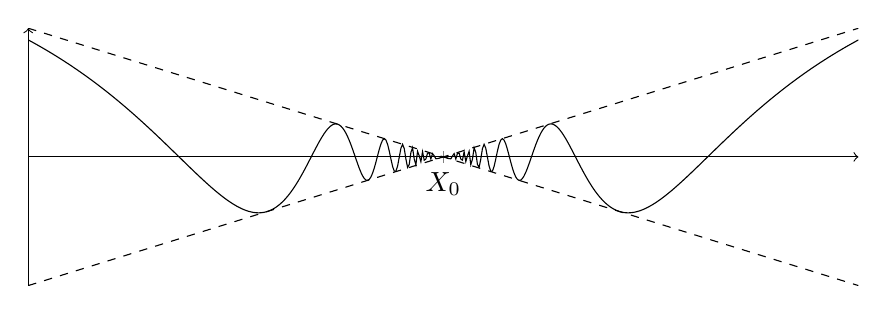
\begin{tikzpicture}
        \begin{axis}[
            width = \textwidth,
            height = 0.4\textwidth,
            xtick = {0}, ytick = \empty,
            xticklabels = {$X_0$},
            ymin = -0.5, ymax = 0.5,
            axis x line = center,
            axis y line = left,
            axis line style = {->},
            domain = -0.5:0.5,
        ]
         
        \addplot[color = black, samples = 500] {x*sin(deg(1/x))};
        \addplot[color = black, dashed] {x};
        \addplot[color = black, dashed] {-x};
        \end{axis}
    \end{tikzpicture}
        
    $f(X_n) = \underbrace{X_n}_{\to 0} \cdot \underbrace{\sin\qt{\frac{1}{X_n}}}_{\text{beschränkt}}$
    für jede Nullfolge $(X_n)$ in $\IR \setminus \{0\}$

    $
        \imp \tilde{f}(x) = \begin{cases}
            x \cdot \sin\qt{\frac{1}{x}} & x \neq 0 \\
            0 & x = 0
        \end{cases}    
    $ stetige Fortsetzung.

    \item $f: \IR \setminus \{0\} \to \IR \quad f(x) = \sin(x) \cdot \frac{1}{x}$
    
    Wir zeigen später mit L'Hopital, dass $\lim\limits_{x \to 0} f(x) = 1$

\end{enumerate}

\subsection{Satz: Zwischenwertsatz von Bolzano (Nullstellensatz)}

$f: [a, b] \to \IR$ stetig, $f(a) \cdot f(b) < 0$.
Dann: Es gibt $c \in [a, b]$ mit $f(c) = 0$.

\textbf{Beweis: }
$f(a) \cdot f(b) < 0$ bedeutet, dass $f(a)$ und $f(b)$ unterschiedliche Vorzeichen haben.

Beweis für $f(a) < 0, f(b) > 0$ (Anderer Fall analog)

Anschaulich klar, da $f$ keine Sprungstelle hat.

\textbf{Bisektionsverfahren: }

Start $[a_1, b_1] := [a, b]$

1. Schritt: Halbiere $[a_1, b_1]$
\begin{itemize}
    \item Berechne $y_1 = f\qt{\frac{a_1 + b_1}{2}}$
    \item Fallunterscheidung:
    \begin{itemize}
        \item $y_1 = 0$: Fertig
        \item $y_1 > 0$:
            Neues Intervall $[a_2, b_2] := [a_1, \frac{a_1 + b_1}{2}]$
        \item $y_1 < 0$:
            Neues Intervall $[a_2, b_2] := [frac{a_1 + b_1}{2}, b_1]$
    \end{itemize}
    \item Es gilt:
    \begin{itemize}
        \item $[a_2, b_2]$ halb so groß wie $[a_1, b_1]$
        \item $f(a_2) < 0, f(b_2) > 0$
    \end{itemize}
\end{itemize}
2. Schritt: Wende Schritt 1 auf $[a_2, b_2]$ an, erhalte $y_2$ und $[a_3, b_3]$

Usw...


\ifdefined\MAINDOC\else
\end{document}
\fi
    \ifdefined\MAINDOC\else
\documentclass[10pt, a4paper, fleqn]{article}
\usepackage{base}

\begin{document}
    \title{Skript Mathe 2}
    \date{11. Juni 2018}
    \maketitle
\fi

Erhalte Intervallschachtelung $[a_n, b_n]$ mit
\begin{itemize}
    \item $a_n \nearrow, b_n \searrow$
    \item $b_n - a_n \to 0$
    \item $a_n \leq b_n$
\end{itemize}
\[
    \underset{1.26}{\imp} \lim_{n \to \infty} a_n = \lim_{n \to \infty} b_n = c
\]

Es ist $f(a_n) \leq 0, f(b_n) \geq 0 \ \forall n \in \IN$.
Da $f$ stetig, gilt:
\[\begin{aligned}
    & \underbrace{\lim_{n \to \infty} f(a_n)}_{\leq 0} = f(c) \\
    & \underbrace{\lim_{n \to \infty} f(b_n)}_{\geq 0} = f(c) \\
    & \imp f(c) = 0 \qed
\end{aligned}\]

Dieses Verfahren verwendet man auch zur Nullstellenberechnung.

\subsection{Satz: Zwischenwertsatz allgemein}
$f: [a, b] \to \IR$ stetig, $y$ sei eine Zahl zwischen $f(a)$ und $f(b)$.

Dann gibt es $\overline{x} \in [a, b]$ mit $f(\overline{x}) = y$.

\textbf{Beweis: }

Ohne Beschränkung der Allgemeinheit (o.B.d.A)
\[
    f(a) \geq y \geq f(b)    
\]
Setze $g: [a, b] \to \IR, x \to f(x) - y \imp$
\begin{itemize}
    \item $g(a) = f(a) - y \geq 0$
    \item $g(b) = f(b) - y \geq 0$
    \item $g$ stetig
\end{itemize}
\[
    \imp \exists \ \overline{x} \in [a, b]: y(\overline{x}) = 0 \imp f(\overline{x}) = g \qed    
\]

\subsection{Satz}
Sei $D$ ein Intevall, $f: D \to \IR$ stetig. Dann gilt:
\begin{enumerate}[1.]
    \item $f(D)$ Intervall oder enthält genau ein Element
    \item $f$ injektiv $\eqv$ $f$ streng monoton
\end{enumerate}
\textbf{Beweis: }

\begin{enumerate}
    \item Falls $f(D)$ nur ein Element enthält: fertig \checkmark

    Enthalte $f(D)$ mindestens 2 Elemente $y_1 < y_2.$
    \[\begin{aligned}
        &\imp \exists x_1, x_2 \in D: & f(x_1) = y_1 \\
        &&f(x_2) = y_2 \\
        &\imp x_1 \neq x_2
    \end{aligned}\]
    Zeige: Jedes $y \in [y_1, y_2]$ ist in $f(D)$:

    Falls $x_1 < x_2$, gibt es wegen 5.24 ein $x \in \underbrace{[x_1, x_2]}_{\subseteq D}$ 
    mit $f(x) = y$. \\
    Analog für $x_2 < x_1$.
    \[
        \imp y \in f(D) \imp f(D) \text{ Intervall.}    
    \]

    \item $(\Leftarrow)$: Hierzu braucht man die Stetigkeit nicht:

    $f$ streng monoton wachsend (fallend). Sei $x = y$. \\
    O.B.d.A: $x < y$
    \[
        \imp f(x) \underset{\hbox{(>)}}{<} f(y) \imp f(x) \neq f(y)    
    \]
    $(\Rightarrow)$: Hierzu braucht man die Stetigkeit: 
    
    Kontraposition: Sei $f$ nicht
    streng monoton.
    \[\begin{aligned}
        &\imp \exists x < y < z \in D: f(x) < f(y) \text{ und } f(y) \geq f(z) \\ 
        &(\text{oder } f(x) \geq f(y) \text{ und } f(y) \leq f(z)).
    \end{aligned}\]
    $\underset{5.24}{\imp}$ \begin{itemize}
        \item $f$ nimmt in $[x, y]$ jeden Wert zwischen $f(x)$ und $f(y)$ an.
        \item $f$ nimmt in $[y, z]$ jeden Wert zwischen $f(y)$ und $f(z)$ an.
    \end{itemize}
    $\imp$ Mindestens ein Wert wird doppelt getroffen. $\qed$
\end{enumerate}

\subsection{Satz}
Sei $D \subseteq \IR$ Intervall und $f: D \to f(D)$ bijektiv und stetig.

Dann gilt für die Umkehrfunktion $f^{-1}$
\begin{enumerate}[1.]
    \item $f^{-1}$ ist im selben Sinne streng monoton wie $f$
    \item $f^{-1}$ ist stetig
\end{enumerate}

\textbf{Beweis: }
\begin{enumerate}[1.]
    \item $f$ stetig und injektiv $\underset{5.25/2.}{\imp} f$ streng monoton. \\
    Zeige Aussage für $f$ streng monoton wachsend:

    Für $y_1 < y_2; \ y_1, y_2 \in f(D)$ gibt es $x_1 \neq x_2$ mit \\
    $f(x_1) = y_1, f(x_2) = y_2$.

    %TODO Underset
    Es gilt: $\underbrace{y_1}_{= f(x_1)} < \underbrace{y_2}_{= f(x_2)} 
    \underset{\substack{f \text{ streng monoton} \\ \text{ wachsend}}}{\eqv} x_1 < x_2$

    \[\begin{aligned}
        &\eqv f^{-1}(y_1) < f^{-1}(y_2) \\
        &\imp f^{-1} \text{ streng monoton wachsend}
    \end{aligned}\]

    \item $f$ stetig und injektiv $\underset{5.25}{\imp} f(D)$ Intervall, 
    $f$ streng monoton.
\end{enumerate}

\textbf{Annahme: } $f$ streng monoton waschend.

Sei $y_0 \in f(D)$. z.Z: $f^{-1}$ stetig in $y_0$.
Setze $x_0 := f^{-1}(y_0)$.

1. Fall: $x_0$ kein Randpunkt von $D$. 

Mit $\epsilon$--$\delta$--Kriterium:
Sei $\epsilon > 0$, so dass $(x_0 - \epsilon, x_0 + \epsilon) \subseteq D$.

$f$ streng monoton wachsend
\[\begin{aligned}
    &\imp f(x_0 - \epsilon) < y_0 < f(x_0 + \epsilon) \\
    &\imp (f(x_0 - \epsilon), f(x_0 + \epsilon)) \subseteq f(D)
\end{aligned}\]
da $f(D)$ Intevall.

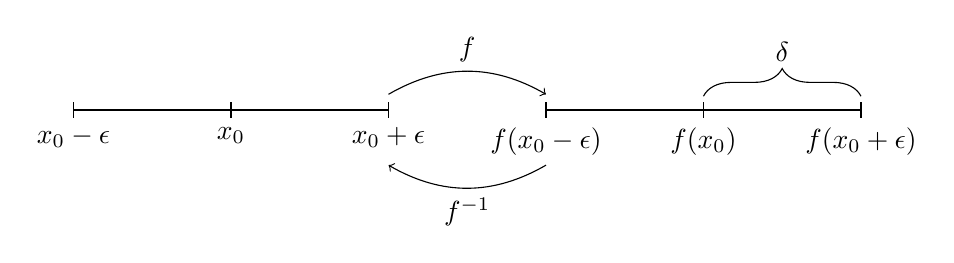
\begin{tikzpicture}
    \draw (0, 0) -- (4, 0);
    \draw (6, 0) -- (10, 0);

    \foreach \x/\xtext in {
        0/$x_0 - \epsilon$, 2/$x_0$, 4/$x_0 + \epsilon$,
        6/$f(x_0 - \epsilon)$, 8/$f(x_0)$, 10/$f(x_0 + \epsilon)$}
        \draw (\x, 0.1) -- (\x, -0.1) node[below] {\xtext};

    \draw[decorate, decoration = {brace, amplitude = 10pt, raise = 5pt}] (8, 0) -- node[above = 14pt] {$\delta$} (10, 0);

    \draw[->] (4, 0.2) to[out = 30, in = 150] node[midway, above] {$f$} (6, 0.2);
    \draw[->] (6, -0.7) to[out = -150, in = -30] node[midway, below] {$f^{-1}$} (4, -0.7);
\end{tikzpicture}

Sei $\delta := \min\{|y_0 - f(x_0 + \delta)|, |y_0 - f(x_0 - \epsilon)|\}$

$\imp f^{-1}((y_0 - \delta, y_0 + \delta)) \subseteq (x_0 - \epsilon, x_0 + \epsilon)$

D.h.: $|y-y_0| < \delta \imp |\underbrace{f^{-1}(y)}_{x} - \underbrace{f^{-1}(y_0)}_{x_0}| < \epsilon$

Analog für streng monoton fallend.

2. Fall: $x_0$ linker Randpunkt von $D$: \\
Analog zu Fall 1 mit $[x_0, x_0 + \epsilon] \subseteq D$

3. Fall: $x_0$ rechter Randpunkt von $D$: \\
Analog zu Fall 2. $\qed$

\subsection{Bemerkung}
Wegen 5.26 und 5.21 sind Wurzelfunktionen, $\arcsin, \arccos, \arccotan$ und Logarithmen stetig.

\subsection{Satz: $\exp(1) = e$}

\textbf{Beweis: } Es ist $\lim\limits_{x \to 0} \frac{\exp(x) - 1}{x} = 1$ \\
(Beweis der Gleichung zeigen wir nicht)

Substitution: \[\begin{aligned}
    &y = \exp(x) - 1 \eqv \\
    &x = \ln(y + 1) \\
    &\underset{\substack{
        \text{weil } \exp \\
        \text{stetig ist}
    }}{\imp} \lim_{y \to 0} \ln((y + 1)^{\frac{1}{y}}) = \lim_{y \to 0} \frac{1}{y} \ln (y + 1) \\
    &[y \to 0 \eqv x \to y] \\
    &= \lim \frac{x}{\exp(x) - 1} = 1
\end{aligned}\]

Wende auf Gleichung $\exp$ an

Da $\exp$ stetig: $\lim\limits_{y \to 0}(y + 1)^{\frac{1}{y}} = \exp(1)$ \\
Insbesondere für $Y_n = \frac{1}{n}: \underbrace{\lim\limits_{n \to \infty} \qt{1 + \frac{1}{n}}^n}_{=e \ (1.28)} = \exp(1)
\qed$

\ifdefined\MAINDOC\else
\end{document}
\fi
    \ifdefined\MAINDOC\else
\documentclass[10pt, a4paper, fleqn]{article}
\usepackage{base}

\begin{document}
    \title{Skript Mathe 2}
    \date{13. Juni 2018}
    \maketitle
\fi
\subsection{Bemerkung}
Wegen 5.28 ist $e \approx 2,718$ die Basis zur Exponentialfunktion $\exp(x)$. \\
Man erhält $e^x = \underset{\text{4.11a2}}{\exp}(x \cdot \ln(\underset{= \exp(1)}{e})) = \exp(x)$

Siehe auch 4.11 Exkurs

\subsection{Minimax-Theorem von Weierstraß}

Jede stetige Funktion $f: [a, b] \to \IR$ besitzt sowohl ein Minimum als auch ein Maximum,
d.h:
\[
    \exists x_*, x^* \in [a, b]: f(x_*) \leq f(x) \leq f(x^*) \quad \forall x \in [a, b]    
\]
\textbf{Beweis: } Genügt z.Z: $f$ hat Maximum (Minimum analog).

Sei $s := \sup f([a, b])$ (kleinste obere Schranke des Bildes von $f$).

Zeige: $s < \infty$ und $s \in f([a, b])$.

Sei $(X_n)$ Folge in $[a, b]$ mit $f(X_n) \to s$.

$(X_n)$ beschränkt $\imp \exists$ konvergente Teilfolge $(X_{n_j})$ mit
$\lim\limits_{i \to \infty} X_{n_j} = \tilde{x}, \tilde{x} \in [a, b]$, da
$[a, b]$ abgeschlossen, ist $f$ stetig.

$\imp \lim\limits_{j \to \infty} f(X_{n_j}) = s = f(\tilde{x})$ \\
$\imp s$ Funktionswert von $\tilde{x}$ und somit $f < \infty$ \\
$\imp s \in f([a, b])$ und somit $f(x) \leq s \quad \forall x \in [a, b]$

\subsection{Beispiele}
\begin{enumerate}[a)]
    \item $f(x) = x^2$ auf $[0, 1]$ \\
    $f(x_*) = 0, f(x^*) = 1$

    \item Falls der Definitionsbereich nicht abgeschlossen ist:
    \begin{itemize}
        \item $f(x) = x^2$ besitzt auf $(0, 1)$ weder Minimum noch Maximum.
        \item $f(x) = \frac{1}{x}$ besitzt auf $(0, 1)$ weder Minimum noch Maximum,
        jedoch ist $f(\underbrace{x_*}_{1}) = 1$
    \end{itemize}
    \item $f(x) = \sin(x)$ hat je nach Größe des festgelegten Definitionsbereiches mehrere
    Minimal/-Maximalstellen
\end{enumerate}

\section{Differenzierbare Funktionen}

\subsection{Bemerkung: Tangenten}

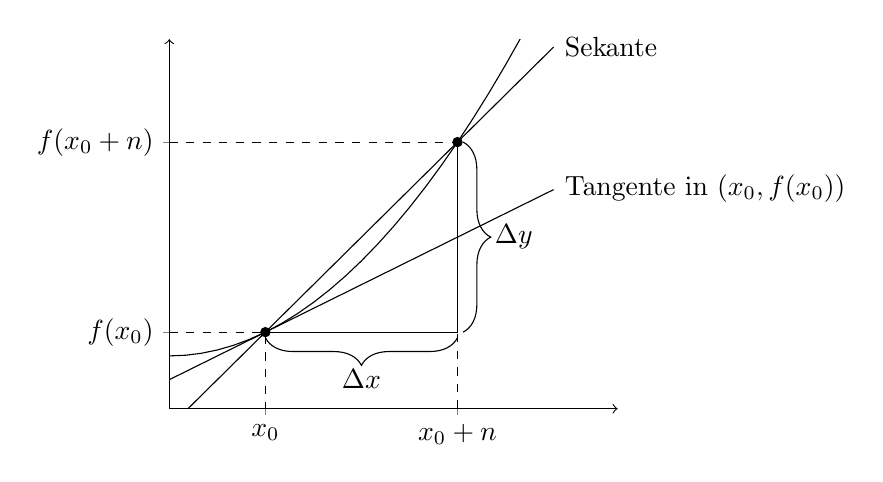
\begin{tikzpicture}[
    declare function = {
        f(\x) = \x^2 + 5;
        t(\x) = 3*x + 2.75;
        s(\x) = 6*x - 1.75;
    }
]
    \begin{axis}[
        width = 0.6\textwidth,
        axis x line = center,
        axis y line = left,
        ymin = 0, ymax = 35,
        xmin = 0, xmax = 7,
        xtick = {1.5, 4.5},
        xticklabels = {$x_0$, $x_0 + n$},
        ytick = {7.25, 25.25},
        yticklabels = {$f(x_0)$, $f(x_0 + n)$},
        axis line style = {->},
        domain = 0:6
    ]
    \addplot[color = black] {f(x)};  
    \addplot[color = black] {t(x)};
    \addplot[color = black] {s(x)};

    \draw (1.5, {f(1.5)}) node[circle, fill = black, scale = 0.4]{};
    \draw (4.5, {f(4.5)}) node[circle, fill = black, scale = 0.4]{};
    \draw (1.5, {f(1.5)}) -- (4.5, {f(1.5)}) -- (4.5, {f(4.5)});
    
    \draw[dashed] (0, {f(1.5)}) -- (1.5, {f(1.5)}) -- (1.5, 0);
    \draw[dashed] (0, {f(4.5)}) -- (4.5, {f(4.5)});
    \draw[dashed] (4.5, 0) -- (4.5, {f(1.5)});

    \draw[decorate, decoration = {brace, amplitude = 10pt, raise = 2pt}] 
        (4.5, {f(1.5)}) -- (1.5, {f(1.5)}) node[midway, below = 10pt]{$\Delta x$};
    \draw[decorate, decoration = {brace, amplitude = 10pt, raise = 2pt}] 
        (4.5, {f(4.5)}) -- (4.5, {f(1.5)}) node[midway, right = 10pt]{$\Delta y$};

    \end{axis}
    \draw (4.9, 2.8) node[right] {Tangente in $(x_0, f(x_0))$};
    \draw (4.9, 4.6) node[right] {Sekante};
\end{tikzpicture}

Die Sekante durch die Punkte $(x_0, f(x_0))$ und \\
$(x_0 + h, f(x_0 + h))$ hat die Steigung 
\[
    \frac{\Delta x}{\Delta y} =
    \frac{f(x_0 + h) - f(x_0)}{h} \ \widehat{=} \text{ Differenzenquotient}
\]
Je kleiner $h$, desto besser nähert sich die Sekante an die Tangente
$(x_0, f(x_0))$ an. Daraus ergibt sich die Tangentensteigung:
$\lim\limits_{h \to 0} \dfrac{f(x_0 + h) - f(x_0)}{h}$, falls der Grenzwert existiert.

\bigskip
In diesem Kapitel sei $I$ immer offenes Intervall.
\subsection{Definition: Ableitung}
Sei $f: I \to \IR, x \in I$
\begin{enumerate}[1.]
    \item $f$ heißt differenzierbar in $x_0$, falls
    $\lim\limits_{h \to 0} \dfrac{f(x_0 + h) - f(x_0)}{h}$ existiert. Dieser
    Grenzwert heißt die Ableitung von $f$ in $x_0$ und wird mit $f'(x_0)$ oder
    $\dfrac{d}{dx} f(x_0)$ bezeichnet.

    \item Ist $f$ differenzierbar in jedem $x_0 \in I$, so heißt $f$ differenzierbar
    (auf $I$) und man nennet $f': I \to \IR, x \mapsto f'(x)$ die Abbildung von $f$.
\end{enumerate}

\subsection{Bemerkung}

Setzt man in 6.2/1 $x = x_0 + h$, so erhält man für den Grenzwert des
Differenzenquotienten $\lim\limits_{x \to x_0} \dfrac{f(x) - f(x_0)}{x - x_0}$.

\subsection{Beispiele}

\begin{enumerate}[a)]
    \item $f(x) = c$ für $x \in \IR$:
    \[
        \lim_{h \to 0} \frac{c - c}{h} = 0 = f'(x) \quad \forall x \in \IR
    \]

    \item $(x^2)' = 2x \quad \forall x \in \IR:$
    \[
        \frac{(x + h)^2 - x^2}{h} = \frac{\cancel{x^2} + 2x\bcancel{h} + h^2 - \cancel{x^2}}{\bcancel{h}} = 2x + h \to 2x
    \]

    \item $(x^n)' = nx^{n-1} \quad \forall x \in \IR, n \in \IN:$
    \[\begin{aligned}
        &\frac{(x + h)^n - x^n}{h} = \frac{\sum_{k=0}^n \qt{\binom{n}{k} x^{n - k} h^k} - x^n}{h} \\
        &= \sum_{k=1}^n \qt{\binom{n}{k} x^{n - k} h^{k-1}} - \underbrace{x^n}_{\mathclap{\substack{\to 0 \text{ für } \\ h \to 0, \ k \neq 1}}} \\
        &\to nx^{n-1} \text{ für } h \to 0
    \end{aligned}\]

    \item $\qt{\frac{1}{x}}' = -\frac{1}{x^2} \quad \forall x \neq 0:$
    \[\begin{aligned}
        &\frac{\frac{1}{x+h} - \frac{1}{x}}{h} = \frac{x - (x + h)}{(x + h)x \cdot h}
        = \frac{-1}{x \cdot (x + h)} \\
        &\to -\frac{1}{x^2} \text{ für } h \to 0
    \end{aligned}\]

    \item Analog zu c) erhält man
    \[
        \qt{\frac{1}{x^n}}' = \frac{-n}{x^{n+1}} \quad \forall x \neq 0    
    \]

    \item $(e^x)' = e^x$.

    Es ist $e^x = \exp(x)$ (5.29). Wir benutzen in Beweis von 5.28 \\
    $\lim\limits_{h \to 0} \dfrac{\exp(h) - 1}{h} = 1$. Damit gilt:
    \[\begin{aligned}
        &\frac{\exp(x + h) - \exp(x)}{h} = \frac{\exp(x) \exp(h) - \exp(x)}{h} \\
        & = \exp(x) \cdot \frac{\exp(h) - 1}{h} \xrightarrow[h \to 0]{} \exp(x)
    \end{aligned}\]

    \item $(\sin x)' = \cos(x), \ (\cos x)' = \sin(x) \quad \forall x \in \IR$

    Ohne Beweis. Man zeigt dies, indem man $\sin$ und $\cos$ mit Hilfe von $\exp$ darstellt
    ($\to$ Mathe III)
\end{enumerate}

\subsection{Satz: Lineare Approximation}

Sei $f: I \to \IR, x_0 \in I$.

Dann sind äquivalent:
\begin{enumerate}[1.]
    \item $f$ ist in $x_0$ differenzierbar
    \item Es gibt eine Funktion $R: I \to \IR$, stetig in $x_0$, $R(x_0) = 0$ und ein
    $m \in \IR$, so dass
    \[
        f(x) = f(x_0) + \underbrace{m(x - x_0)}_{\mathclap{\text{Tangente an $f$ in $x_0$}}}
        + R(x)(x - x_0) \quad (*)    
    \]
\end{enumerate}

Bemerkung: \begin{itemize}
    \item In $\IR: m = f'(x_0)$
    \item 2. heißt: $f$ ist in $x_0$ durch eine Gerade (Tangente) approximierbar.
\end{itemize}

\ifdefined\MAINDOC\else
\end{document}
\fi
    \ifdefined\MAINDOC\else
\documentclass[10pt, a4paper, fleqn]{article}
\usepackage{base}

\begin{document}
    \title{Skript Mathe 2}
    \date{18. Juni 2018}
    \maketitle
\fi
\textbf{Beweis: } $\boxed{1. \Rightarrow 2.}$ Sei $f$ in $x_0$ differenzierbar.
\[\begin{aligned}
    &\text{Setze } R(x) = \begin{cases}
        \dfrac{f(x) - f(x_0)}{x - x_0} - f'(x_0) & x \neq x_0 \\
        0 & x = x_0
    \end{cases} \\
    &\imp \lim_{n \to 0} R(x_0 + h) = \lim_{n \to 0} \frac{f(x_0 + h) - f(x_0)}{h} - f'(x_0) \\
    &= R(x_0) = 0
\end{aligned}\]
$\imp R$ stetig in $x_0, R(x_0) = 0$ und (*) ist erfüllt für $m = f'(x_0)$.
\bigskip

$\boxed{2. \Rightarrow 1.}$ Gelte (*) für ein $m \in \IR$ und eine in $x_0$ stetige Funktion 

$R: I \to \IR, R(x_0) = 0$.
\[\begin{aligned}
    &f(x_0 + h) = f(x_0) + m \cdot h + R(x_0 + h) \cdot h \\
    &\underset{h \neq 0}{\eqv} \frac{f(x_0 + h) - f(x_0)}{h} = m + R(x_0 + h) \\
    &\xrightarrow[h \to 0]{} \lim_{h \to 0} \frac{f(x_0 + h) - f(x_0)}{h} = m + \underbrace{R(x_0)}_{= 0} \\
\end{aligned}\]
da $R(x_0) = 0$ und stetig in $x_0 \qed$

\subsection{Satz}
Wenn $f$ differenzierbar in $x_0 \in I \imp f$ stetig.

\textbf{Beweis: } Folge aus 6.5/2 (*), da $f$ Summe in $x_0$ stetiger Funktionen.

\subsection{Bemerkung}
Die Umkehrung von 6.6 gilt nicht. In $x_0 = 0$ hat $f'(x_0) = |x|$ einen Knick:
\begin{itemize}
    \item $\lim\limits_{n \to 0^-} \dfrac{|0 + h| - h}{h} = \lim\limits_{h \to 0} \dfrac{-h}{h} = -1$
    \item $\lim\limits_{n \to 0^+} \dfrac{|0 + h| - h}{h} = \lim\limits_{h \to 0} \dfrac{h}{h} = 1$
\end{itemize}
$\underset{5.12}{\imp}$ In $x_0 = 0$ existiert keine Ableitung.

\section*{Rechenregeln}

\subsection{Satz: Ableitungsregeln}
$f, g: I \to \IR$ differenzierbar in $x \in I$.

Dann sind auch $c \cdot f$ (für $c \in \IR$), $f \pm g, f \cdot g$ und \\
$\frac{f}{g}$ (für $g(x) \neq 0$) differenzierbar in x mit:
\begin{enumerate}[a)]
    \item $(c \cdot f)'(x) = c \cdot f'(x)$
    \item $(f \pm g)'(x) = f'(x) \pm g'(x)$
    \item Produktregel:
    
    $(f \cdot g)'(x) = f'(x) \cdot g(x) + f(x) \cdot g'(x)$
    \item Quotientenregel:

    $\qt{\frac{f}{g}}'(x) = \dfrac{f'(x) \cdot g(x) - f(x) \cdot g'(x)}{g^2(x)}$
\end{enumerate}

\textbf{Beweis: }
\begin{enumerate}
    \item[a, b)] Übung
    \item[c)]
    \[\begin{aligned}
        &\frac{(fg)(x + h) - (fg)(x)}{h} \\
        &= \frac{f(x + h)g(x + h) \overbrace{-f(x)g(x + h) + f(x)g(x + h)}^{= 0} - f(x)g(x)}{h} \\
        &= \frac{(f(x + h)- f(x)) \cdot g(x + h)}{h} + \frac{f(x) \cdot (g(x + h) - g(x))}{h} \\
        &\xrightarrow[h \to 0]{} f'(x) \cdot g(x) + f'(x) \cdot g'(x) \quad \text{ (da $g$ stetig)}
    \end{aligned}\]
    \item[d)]
    \[
        \frac{\qt{\frac{f}{g}}(x + h) - \qt{\frac{f}{g}}(x)}{h} =
        \frac{f(x+h)g(x) - f(x) - g(x + h)}{h \cdot g(x + h) \cdot g(x)}
    \]
    Schiebe wie in c) im Zähler $-f(x + h) g(x + h) + f(x + h) g(x + h)$ ein und erhalte
    mit $h \to 0$ die Behauptung. $\qed$
\end{enumerate}

\subsection{Beispiele}
\begin{enumerate}[a)]
    \item Wegen 6.8a,d) ist jedes Polynom und jede rationale Funktion differenzierbar.
    \item $(4x^3 + 7x + 5)' = 12x^2 + 7$
    \item $\qt{\dfrac{\sin x}{x}}' = \dfrac{\cos x \cdot x - \sin x}{x^2} \quad (x \neq 0)$
    \item $(\tan x)' = \dfrac{\cos^2 x + \sin^2 x}{\cos^2 x} = \dfrac{1}{\cos^2 x}$
\end{enumerate}

\subsection{Satz: Kettenregel}
Die Verknüpfung $f \circ g$ zweier differenzierbarer Funktionen $f, g$ ist differenzierbar und
es gibt $(f \circ g)' = (f' \circ g) \cdot g'$ bzw $\frac{d}{dx} f(g(x)) = f'(g(x)) \cdot g'(x)$.

\textbf{Beweis: } Mit Substitution:

$\tilde{x} = g(x), \ \tilde{h} = g(x + h) - g(x)$

Es gilt: $h \to 0 \imp \tilde{h} \to 0$ da $g$ stetig. Damit ist
\[\begin{aligned}
    &\frac{f(g(x + h)) - f(g(x))}{h} \\
    &= \frac{f(g(x + h) - g(x) + g(x)) - f(g(x))}{g(x + h) - g(x)} \cdot \frac{g(x + h) - g(x)}{h} \\
    &= \frac{f(\tilde{x} + \tilde{h}) - f(\tilde{x})}{\tilde{h}} \cdot \frac{g(x + h) - g(x)}{h} \\
    &\xrightarrow[h \to 0]{} f'(\tilde{x}) \cdot g'(x) = f'(g(x)) \cdot g'(x) \qed
\end{aligned}\]

\subsection{Beispiel}
\[
    (\overbrace{\sin (\underbrace{5x^2}_{g})}^{f \circ g})' = \underbrace{10x}_{g'} \underbrace{\cdot \cos(5x^2)}_{f' \circ g}
\]

\subsection{Veranschaulichung zur Ableitung der Umkehrfunktion}
\begin{tikzpicture}[
    declare function = {
        f(\x) = 3.289562 + 0.6189274*\x + 0.09662097*\x^2 + 0.01076239*\x^3;
        t(\x) = 1.304*\x + 2.349;
        t2(\x) = -0.766871*(2.349 - \x);
    }
]
    \begin{axis}[
        width = \textwidth,
        height = \textwidth,
        axis x line = center,
        axis y line = center,
        xtick = {-7}, ytick = {-7},
        xticklabels = \empty, yticklabels = \empty,
        ymin = -12, ymax = 12,
        xmin = -12, xmax = 12,
        axis line style = {->},
        domain = -12:12,
        clip = false
    ]
    \addplot[color = black, domain = -11:7.4] {t(x)};
    \addplot[color = black] {t2(x)};
    \addplot[dashed, color = black] {x};
    
    % Not true, bad
    %\draw (-7, 0.3) -- (-8, 2) node[yshift = 4pt] {$m = 0$};
    %\draw (0.3, -7) -- (2, -8) node[right] {$m'$ unendlich groß};

    \draw (-12.5, -9.5) node {$f$};
    \draw (-7, -12.5) node {$f^{(-1)}$};

    \draw[->] (1.8, 10.5) to [out = 150, in = 60] (-4, 8) node[left] {$m = \dfrac{\Delta x}{\Delta y}$};
    \draw[->] (10.5, 1.8) to [out = -30, in = -170] (14, 1) node[right] {$m' = \dfrac{\Delta x}{\Delta y} = \dfrac{1}{m}$};

    \coordinate (A) at (2.5, {t(2.5)});
    \coordinate (B) at (2.5, {t(6)});
    \coordinate (C) at (6, {t(6)});

    \coordinate (D) at ({t(2.5)}, {t2(t(2.5))});
    \coordinate (E) at ({t(6)}, {t2(t(2.5))});
    \coordinate (F) at ({t(6)}, {t2(t(6))});

    \draw (A) node[circle, fill = black, scale = 0.3]{};
    \draw (D) node[circle, fill = black, scale = 0.3]{};

    \draw (A) -- (B) -- (C);
    \draw[decorate, decoration = {brace, amplitude = 10pt, raise = 2pt}] (A) -- (B) node[midway, left, xshift = -10pt] {$\Delta y$};
    \draw[decorate, decoration = {brace, amplitude = 10pt, raise = 2pt}] (B) -- (C) node[midway, above, yshift = 10pt] {$\Delta x$};

    \draw (D) -- (E) -- (F);
    \draw[decorate, decoration = {brace, amplitude = 10pt, raise = 2pt}] (F) -- (E) node[midway, right, xshift = 10pt] {$\Delta x$};
    \draw[decorate, decoration = {brace, amplitude = 10pt, raise = 2pt}] (E) -- (D) node[midway, below, yshift = -10pt] {$\Delta y$};


    \end{axis}

    % Second axis so that we can mirror without running into problems
    \begin{axis}[
        hide axis,
        width = \textwidth,
        height = \textwidth,
        ymin = -12, ymax = 12,
        xmin = -12, xmax = 12,
        domain = -12:12,
    ]
    \addplot[color = black, domain = -12:6] {f(x)};
    \addplot[rotate = -90, xscale = -1, color = black, domain = -12:6] {f(x)};
    \end{axis}

\end{tikzpicture}

\[\begin{aligned}
    &m = f'(x_0) \neq 0 \imp (f^{-1}(y_0))' = m' = \frac{1}{m} \\
    &= \frac{1}{f'(x_0)} = \frac{1}{f'(f^{-1} (y_0))}
\end{aligned}\]

\subsection{Satz: Ableitung der Umkehrfunktion}
$I, J$ offene Intervalle, $f: I \to J$ differenzierbar in $x_0 \in I$ mit
$f'(x_0) \neq 0$. Dann:

$f^{-1}: y \to I$ differenzierbar in $y_0 = f(x_0)$ mit $(f^{-1}(y_0))' = \dfrac{1}{f'(x_0)} = \dfrac{1}{f'(f^{-1}(x_0))}$

\textbf{Beweis: } Sei $t = f(x_0 + h) - f(x_0) \quad (*)$

Es gilt: $h \to 0 \eqv t \to 0$
\[\begin{aligned}
    &\frac{1}{\dfrac{f(x_0 + h) - f(x_0)}{h}} \overset{(*)}{=} \frac{x_0 + h - x_0}{t} \\
    & = \frac{f^{-1}(f(x_0 + h)) - f^{-1}(f(x_0))}{t} \overset{(*)}{=} \frac{f^{-1}(f(x) + t) - f^{-1}(f(x))}{t} \\
    &\xrightarrow[h \to 0]{} \frac{1}{f'(x_0)} = \frac{1}{f'(f^{-1}(y_0))} \qed
\end{aligned}\]

\ifdefined\MAINDOC\else
\end{document}
\fi
    \ifdefined\MAINDOC\else
\documentclass[10pt, a4paper, fleqn]{article}
\usepackage{base}

\begin{document}
    \title{Skript Mathe 2}
    \date{20. Juni 2018}
    \maketitle
\fi

\subsection{Beispiele}
\begin{enumerate}[a)]
    \item Für $f(x) = x^n$ ist $f^{-1} (y) = \sqrt[n]{y}$ \\
    $\imp$ Ableitung von $f^{-1}$ wird in $y = f(0) = 0$ unendlich
    groß, da $f'(0) = 0$
    \[
        (f^{-1}(y))' = \frac{1}{n(\sqrt[n]{y})^{n+1}} = \frac{1}{n\sqrt{y^{n-1}}}
        \quad \text{Für $y \neq 0$}
    \]
    \begin{minipage}{0.6\textwidth}
        \item $\sin: (-\frac{\pi}{2}, \frac{\pi}{2}) \to (-1, 1)$
        
        Sei $y = \sin x, \ y \in (-1, 1)$
        \[
            \arcsin' y = \frac{1}{\cos x} = \frac{1}{\sqrt{1 - \sin^2 x}} =
            \frac{1}{\sqrt{1 - y^2}}
        \]
    \end{minipage}
    \begin{minipage}{0.4\textwidth}
        \begin{tikzpicture}
            \begin{axis}[
                width = \textwidth,
                axis x line = center,
                axis y line = center,
                ytick = \empty,
                xtick = {-90, 90},
                xticklabels = {$-\dfrac{\pi}{2}$, $\dfrac{\pi}{2}$},
                domain = -100:100
            ]
            \addplot[color = black] {sin(x)};
            \end{axis}
        \end{tikzpicture}
    \end{minipage}
    Analog:
    \[\begin{aligned}
        &\bullet& \arccos' y &= \dfrac{1}{\sqrt{1-y^2}} &&y \in (-1, 1) \\
        &\bullet& \arctan' y &= \dfrac{1}{1 + y^2} &&y \in \IR \\
        &\bullet& \arccotan' y &= \dfrac{1}{1 + y^2} &&y \in \IR
    \end{aligned}\]
    
    \item 
    \abovedisplayskip = -\baselineskip % TODO Use this in other places, works really well!
    \[\begin{aligned}
        f &: \IR \to \IR_{> 0} &&f(x) = e^x \\
        f^{-1} &: \IR \to \IR  &&f(y) = \ln y
    \end{aligned}\]
    \[\imp \ln' y = \frac{1}{e^{\ln y}} = \frac{1}{y}\]
    \[\begin{aligned}
        \imp \ln(|y|)' &= \begin{cases}
            \frac{1}{y} & y > 0 \\
            (-1) \cdot \frac{1}{-y} & y < 0 \text{ (Kettenregel)}
        \end{cases} \\
        &= \frac{1}{y} \text{ für } y \neq 0
    \end{aligned}\]
\end{enumerate}

\subsection{Logarithmische Ableitung}
Für $f: \IR \to \IR \setminus \{0\}, f$ differenzierbar, ist
\[
    (\ln |f(x)|)' = \frac{f'(x)}{f(x)} \quad \text{(6.14c + Kettenregel)}
\]
\textbf{Beispiel: } $f'(x) = e^x \cdot (\sin x + 2) \cdot x^5 \quad x \neq 0 \imp f(x) \neq 0$
\[\begin{aligned}
    &\ln(|f(x)|) = x + \ln(\sin x + 2) + 5 \cdot \ln |x| \\
    &\imp (\ln|f(x)|)' = 1 + \frac{\cos x}{\sin x + 2} + \frac{5}{x} = \frac{f'(x)}{f(x)} \\
    &\imp f'(x) = \qt{1 + \frac{\cos x}{\sin x + 2} + \frac{5}{x}}(e^x(\sin x + 2) x^5) \\
    &= x^4 e^x(x(\sin x + 2)) + x \cdot \cos x + 5 \sin(x + 2) \text{ für } x \neq 0
\end{aligned}\]

\textbf{Bemerkung: }

Man kann zeigen, dass die Ableitung auch auf Funktionen mit Werten in ganz $\IR$
anwendbar ist. Dazu bildet man die stetige Fortsetzung von \\ $f'(x)$ auf $\{x \ | \ f(x) = 0\}$

$\imp$ Beispiel gilt auch für $x = 0$. Dann ist $f'(0) = 0$.

\subsection{Satz: Ableitung elementarer Funktionen}
\begin{itemize}
    \item $(a^x)' = (\ln a) \cdot a^x, a > 0, x \in \IR$
    \item $(x^\alpha)' = \alpha x^{\alpha - 1}, \alpha \in \IR, x > 0$
    \item $(x^x)' = (\ln x + 1) \cdot x^x, x > 0$
\end{itemize}

\textbf{Beweis: }
\[
    (a^x)' = (e^{\ln(a^x)})' = (e^{x \cdot \ln a})' =
    \underset{\mathclap{\text{innere $\cdot$ äußere Ableitung}}}{(\ln a) \cdot (e^{x \cdot \ln(a)})} =
    (\ln a) \cdot a^x 
\]
Rest analog $\qed$

\section*{Kurvendiskussion}
\subsection{Definition: Extremum}

$f: D \to \IR$ besitzt in $x_0 \in D$ ein lokales $\underbrace{\text{Maxmimum (Minimum)}}_{\text{Extremum}}$, \\
wenn es ein Intervall $U = (x_0 - \delta, x_0 + \delta) \subseteq D, \delta > 0$ gibt, so dass

$f(x_0) \underset{\hbox{$(\leq)$}}{\geq} f(x) \quad \forall x \in U$ ($\leftarrow$ Umgebung von $x$)

$f$ besitzt in $x_0 \in D$ ein globales Maxmimum (Minimum),

wenn $f(x_0) \underset{\hbox{$(\leq)$}}{\geq} f(x) \quad \forall x \in D$

\subsection{Notwendige Bedingung für lokale Extrema}
Sei $f: D \to \IR$ differenzierbar in $x_0 \in D$.
Falls $f$ in $x_0$ ein lokales Extremum besitzt, so ist $f'(x_0) = 0$.
\bigskip

\begin{minipage}{0.5\textwidth}
    \begin{center}
        \begin{tikzpicture}
            \begin{axis}[
                width = 0.8\textwidth,
                axis lines* = center,
                ytick = \empty,
                xtick = \empty,
            ]
            \addplot[color = black] {-x^2};
            \draw (0, 0) node[circle, fill = black, scale = 0.3]{};
            \end{axis}
        \end{tikzpicture}

        Differenzierbar  
    \end{center}
\end{minipage}
\begin{minipage}{0.5\textwidth}
    \begin{center}
        \begin{tikzpicture}
            \begin{axis}[
                width = 0.8\textwidth,
                axis y line* = center,
                axis x line = none,
                ytick = \empty,
                xtick = \empty,
            ]
            \addplot[color = black] {-abs(x)};
            \draw (0, 0) node[circle, fill = black, scale = 0.3]{};
            \end{axis}
        \end{tikzpicture}

        Nicht differenzierbar
    \end{center}
\end{minipage}
\bigskip

\textbf{Beweis: } Sei $U = (x_0 - \delta , x_0 + \delta), \delta > 0$ und

$\underbrace{f(x_0) \geq f(x)}_{\text{Maxmimum}} \quad \forall x \in U$.
\begin{itemize}
    \item $f(x_0) \geq f(x_0 + h) \quad \forall h < s$.
    \item $f$ differenzierbar $\imp f'(x_0) = \lim\limits_{h \to 0} \dfrac{f(x_0 + h) - f(x_0)}{h}$
    \[\begin{aligned}
        &\imp \lim_{h \to 0^+} \frac{\overbrace{f(x_0 + h) - f(x_0)}^{\leq 0}}{\boxed{h} > 0} \leq 0 \text{ und } \\
        &\lim_{h \to 0^-} \frac{\overbrace{f(x_0 + h) - f(x_0)}^{\leq 0}}{\boxed{h} < 0} \geq 0 \imp f'(x_0) = 0
    \end{aligned}\]
    Für Minimum Analog $\qed$
\end{itemize}
\subsection{Anmerkung}
$f'(x_0) = 0$ ist notwendige Bedingung aber keine hinreichende Bedingung.

\textbf{Beispiel: }
$f(x) = x^3$ hat in $x = 0$ einen Sattelpunkt mit Steigung $0$.
\bigskip

\begin{minipage}{0.4\textwidth}
    \begin{tikzpicture}
        \begin{axis}[
            width = \textwidth,
            axis lines = center,
            ytick = \empty,
            xtick = \empty,
        ]
        \addplot[color = black] {x^3};
        \end{axis}
    \end{tikzpicture}  
\end{minipage}
\begin{minipage}{0.5\textwidth}
    $f$ hat lokales Extremum $\overset{\hbox{$\cancel{\Leftarrow}$}}{\imp} f'(x_0) = 0$
\end{minipage}

\subsection{Mittelwertsätze, Satz von Rolle (1652--1719)}
\begin{enumerate}[1.]
    \item \text{}\\
    \begin{tikzpicture}[
        declare function = {
            f(\x) = \x * 0.6;
            t(\x) = f(\x) - 3;
        }
    ]
        \begin{axis}[
            unit vector ratio* = 1 1 1, 
            xmin = 0, xmax = 14,
            ymin = -1, ymax = 10,
            axis lines = left,
            xtick = {4, 8, 12},
            xticklabels = {$a$, $\xi$, $b$},
            ytick = {2.4, 7.2},
            yticklabels = {$f(a)$, $f(b)$},
            domain = 0:14,
        ]
        \addplot[color = blue, samples = 2] {t(x)};
        \addplot[color = green!60!black, samples = 2] {f(x)};
        \draw[color = red] plot [smooth, tension = 1] coordinates { 
            (4, {f(4)}) (5.5, 6) (8, {t(8)}) (10, 8) (12, {f(12)})
        };
        \addplot[only marks, mark options = {scale = 0.7}] coordinates {
            (4, {f(4)}) (8, {t(8)}) (12, {f(12)})
        };
        \draw[dashed] (4, -1) -- (4, {f(4)}) -- (0, {f(4)});
        \draw[dashed] (12, -1) -- (12, {f(12)}) -- (0, {f(12)});
        \draw[dashed] (8, -1) -- (8, {t(8)});
        \end{axis}
        \draw (7.7, 3.2) node {Tangente};
    \end{tikzpicture}

    \item \text{}\\
    \hspace*{23pt}
    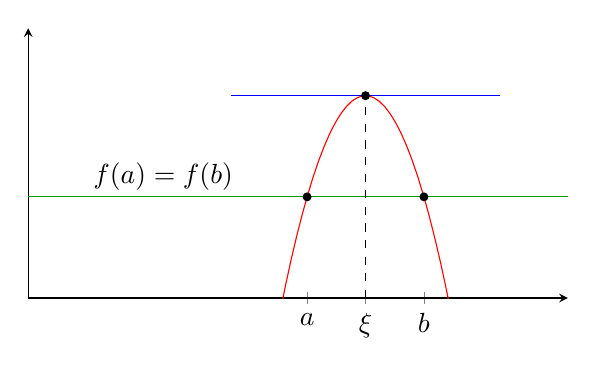
\begin{tikzpicture}[
        declare function = {
            f(\x) = -x^2;
        }
    ]
        \begin{axis}[
            unit vector ratio* = 1 1 1,
            axis lines = left,
            ymin = -6, ymax = 2,
            xtick = {-1.73205080757, 0, 1.73205080757},
            xticklabels = {$a$, $\xi$, $b$},
            ytick = \empty,
            domain = -10:6
        ]
        \addplot[color = red, samples = 50, domain = -4:4] {f(x)};
        \addplot[color = green!60!black, samples = 2] {-3};
        \addplot[color = blue, samples = 2, domain = -4:4] {0};

        \addplot[only marks, mark options = {scale = 0.7}] coordinates {
            ({sqrt(3)}, -3) ({-sqrt(3)}, -3) (0, 0)
        };
        \draw[dashed] (0, -6) -- (0, 0);
        \draw (-6, -2.4) node {$f(a) = f(b)$};
        \end{axis}
    \end{tikzpicture}
\end{enumerate}
Seien $f, g: [a, b] \to \IR$

stetig und differenzierbar in $(a, b), \ g'(x) \neq 0 \quad \forall x \in (a, b)$
\begin{enumerate}[1.]
    \item
    $\imp \exists \xi \in (a, b): \dfrac{f(b) - f(a)}{b - a} = f'(\xi)$

    1. Mittelwertsatz

    \item
    $f(a) = f(b) \imp \exists \xi \in (a, b): f'(\xi) = 0$

    Satz von Rolle

    \item
    $\exists \xi \in (a,b): \dfrac{f(b) - f(a)}{g(b) - g(a)} = \dfrac{f'(\xi)}{g'(\xi)}$

    2. Mittelwertsatz
\end{enumerate}
\textbf{Beweis: }
\begin{enumerate}
    \item [2.] $f$ stetig in $[a, b]$

    $\underset{3.36}{\imp} f$ besitzt Maxmimum $M$ und Minimum $m$ in $[a, b]$.

    D.h: $m \leq f(x) \leq M \quad \forall x \in [a, b]$
\end{enumerate}
\ifdefined\MAINDOC\else
\end{document}
\fi
    \ifdefined\MAINDOC\else
\documentclass[10pt, a4paper, fleqn]{article}
\usepackage{base}

\begin{document}
    \title{Skript Mathe 2}
    \date{25. Juni 2018}
    \maketitle
\fi

\begin{enumerate}
    \item[]
    \begin{enumerate}
        \addtolength{\itemindent}{12pt}
        \item[\underline{1. Fall}:] Beide Extrema werden auf dem Rand angenommen: \\
        $f(a) = f(b) \imp m = M$ \\
        $\imp f$ konstant $\imp f'(\xi) = 0 \quad \forall \xi \in (a, b)$
        \item[\underline{2. Fall:}] Ein Extremum wird auf dem Rand angenommen: \\
        $\imp \exists \xi \in (a, b): f(\xi)$ Extremum $\underset{6.18}{\imp}
        f'(\xi) = 0$.
    \end{enumerate}
    \item[3.]
    Es ist $g(b) \neq g(a)$, denn sonst gäbe es ein $x \in (a, b)$ mit $g'(x) = 0$ (Rolle)

    Hilfsfunktion: $h(x) = f(x) = \dfrac{f(b) - f(a)}{g(b) - g(a)} \cdot g(x)$

    Es ist $h(b) - h(a) = 0$. $h$ stetig auf $[a, b]$ und differenzierbar in $(a, b)$.
    \[\begin{aligned}
        &\underset{\text{Rolle}}{\imp} \exists \xi \in (a, b): h'(\xi) = 0 \\
        &\imp \frac{f'(\xi)}{g'(\xi)} = \frac{f(b) - f(a)}{g(b) - g(a)}
    \end{aligned}\]
    \item[1.] Folgt aus 3. für $g(x) = x$.
\end{enumerate}
\subsection{Monotoniekriterium}
Sei $f: [a, b]$ stetig und auf $(a, b)$ differenzierbar.
\begin{enumerate}[1.]
    \item $f'(x) \underset{\hbox{$(\leq)$}}{\geq} 0 \quad \forall x \in (a, b)
    \eqv f$ monoton $\underset{\hbox{(fallend)}}{\text{wachsend}}$ auf $[a, b]$
    \item $f'(x) \underset{\hbox{$(<)$}}{>} 0 \quad \forall x \in (a, b)
    \underset{\hbox{$\cancel{\Leftarrow}$}}{\imp} f$ streng monoton $\underset{\hbox{(fallend)}}{\text{wachsend}}$ auf $[a, b]$
    \item $f'(x) = 0 \quad \forall x \in (a, b) \eqv f$ konstant auf $[a, b]$
\end{enumerate}
\textbf{Beweis: }
\begin{enumerate}[1.]
    \item $(\Rightarrow):$ Sei $a \leq x_1 < x_2 \leq b$

    $\underset{6.20.1}{\imp} \exists \xi \in (x_1, x_2): f(x_2) - f(x_1) =
    \underbrace{f'(\xi)}_{\geq 0} \cdot \underbrace{(x_2 - x_1)}_{> 0} \geq 0$

    $\imp f(x_1) \leq f(x_2)$

    $(\Leftarrow):$ Sei $f$ monoton wachsend auf $[a, b]$ und differenzierbar in
    $(a, b)$
    \[
        \imp f'(x) = \lim_{h \to 0} \frac{f(x + h) - f(x)}{h}    
    \]\[\begin{aligned}
        &\text{Da} \ \frac{(f(x + h) - f(x)) \geq 0}{h > 0} \geq 0 \text{ für } h < 0 \text{ und } \\
        &\frac{(f(x + h) - f(x)) \leq 0}{h < 0} \leq 0 \text{ ist }
        f'(x) \geq 0 \quad \forall x \in (a, b)
    \end{aligned}\]

    \item[2. + 3.] analog $\qed$
\end{enumerate}
Bemerkung zu 2.: $f(x) = x^3$ ist streng monoton wachsend aber $f'(0) = 0$

\subsection{Satz: Hinreichende Bedingung für lokale Exterma I}

Sei $f: I \to \IR$ differenzierbar und $x_0 \in I, f'(x_0) = 0$
\bigskip
\begin{enumerate}[1.]
    \begin{minipage}{0.5\textwidth}
        \item \raisebox{-\height + \ht\strutbox}{
            \begin{tikzpicture}
                \begin{axis}[
                    width = 1.1\textwidth,
                    unit vector ratio* = 1 1 1, 
                    axis lines = left,
                    ymin = -4, ymax = 1,
                    xmin = -3, xmax = 3,
                    xtick = {-2, 0, 2},
                    ytick = \empty,
                    xticklabels = {$x_0 - \delta$, $x_0$, $x_0 + \delta$},
                    domain = -3:3
                ]
                \addplot[color = black, samples = 50] {-x^2};
                \draw[dashed] (0, -4) -- (0, 0);
                \draw [decorate, decoration = {brace, amplitude = 10pt, raise = 2pt}, yshift = 0pt]
                    (-1.9, -4) -- (-0.1, -4) node [midway, yshift = 20pt] {$f' \geq 0$};
                \draw [decorate, decoration = {brace, amplitude = 10pt, raise = 2pt}, yshift = 0pt]
                    (0.1, -4) -- (1.9, -4) node [midway, yshift = 20pt] {$f' \leq 0$};
                \end{axis}
            \end{tikzpicture}
        }
    \end{minipage}
    \begin{minipage}{0.5\textwidth}
        \item \raisebox{-\height + \ht\strutbox}{
            \begin{tikzpicture}
                \begin{axis}[
                    width = 1.1\textwidth,
                    axis lines = left,
                    ymin = -2, ymax = 2,
                    xmin = -2, xmax = 2,
                    xtick = {-1.25992, 0, 1.25992},
                    ytick = \empty,
                    xticklabels = {$x_0 - \delta$, $x_0$, $x_0 + \delta$},
                    domain = -2:2
                ]
                \addplot[color = black, samples = 50] {x^3};
                \draw[dashed] (0, -4) -- (0, 0);
                \draw [decorate, decoration = {brace, amplitude = 10pt, raise = 2pt}, yshift = 0pt]
                    ({-2^(1/3) + 0.1}, -2) -- (-0.1, -2) node [midway, yshift = 20pt] {$f' > 0$};
                \draw [decorate, decoration = {brace, amplitude = 10pt, raise = 2pt}, yshift = 0pt]
                    (0.1, -2) -- ({2^(1/3) - 0.1}, -2) node [midway, yshift = 20pt] {$f' > 0$};
                \end{axis}
            \end{tikzpicture}
        }
    \end{minipage}
\end{enumerate}
\bigskip

\begin{enumerate}[1.]
    \item
    $f'(y) \underset{\hbox{$(\leq)$}}{\geq} 0 \quad \forall (x_0 - \delta, x_0)$ und \\
    $f'(y) \underset{\hbox{$(\leq)$}}{\geq} 0 \quad \forall (x_0, x_0 + \delta)$ für ein $\delta < 0$

    $\imp f$ hat ein lokales Minimum (Maximum) in $x_0$.

    \item
    $f'(x) < 0 \quad \forall x \in (x_0 - \delta, x_0) \cup (x_0, x_0 + \delta)$

    [1. hat einen Vorzeichenwechsel, 2. nicht]
\end{enumerate}

\textbf{Beweis: } Für lokales Minimum in $x_0$:

Z.z: $f(x) \geq f(x_0) \quad \forall x \in U := (x_0 - \delta , x_0 + \delta)$

Da $x \in U \setminus {x_0} \underset{6.20.1}{\imp} \exists \xi$ zwischen $x$ und $x_0$; \\
$\xi \neq x_0$, so dass $f(x) - f(x_0) = f'(\xi) \cdot (x - x_0)$ (*)

\begin{enumerate}
    \addtolength{\itemindent}{12pt}
    \item[\underline{1. Fall}: ] $x \in (x_0 - \delta, x_0)$
    \[\begin{aligned}
        &\imp x - x_0 < 0, f'(\xi) \leq 0 \\
        &\underset{\text{(*)}}{\imp} f(x) - f(x_0) \geq 0
        \imp f(x) \geq f(x_0)    
    \end{aligned}\]
    \item[\underline{2. Fall}: ] $x \in (x_0, x_0 + \delta)$
    \[\begin{aligned}
        &\imp x - x_0 > 0, f'(\xi) \geq 0 \\
        &\underset{\text{(*)}}{\imp} f(x) - f(x_0) \geq 0
        \imp f(x) \geq f(x_0)    
    \end{aligned}\]
\end{enumerate}
Insgesamt: $f(x) \geq f(x_0) \quad \forall x \in U$

(Rest analog) $\quad \qed$

\subsection{Bemerkung}
\hfill
\begin{minipage}{0.4\textwidth}
    \begin{tikzpicture}
        \begin{axis}[
            width = 1.2\textwidth,
            axis y line = left,
            axis x line = center,
            ymin = -1.5, ymax = 1.5,
            xmin = -1, xmax = 1,
            xtick = {0},
            xticklabels = {$x_0$},
            ytick = \empty
        ]
        \addplot[color = black, samples = 2] {1.7*x};
        \draw[color = black] plot [smooth, tension = 1.2] coordinates {
            (-2, 0) (-1, -1) (1, 1) (2, 0)
        };
        \end{axis}
        \draw (4.5, 2.9) node {$f'$};
    \end{tikzpicture}    
\end{minipage}
\hfill
\begin{minipage}{0.4\textwidth}
    Vorzeichenwechsel von - nach + \\
    $\imp f$ hat Minimum in $x_0$
\end{minipage}
\bigskip

$f'$ weist in $x_0$ einen Vorzeichenwechsel auf, wenn die Steigung von $f'$ in $x_0$
positiv (negativ) ist, d.h. wenn $f''(x_0) > 0 \ (f''(x_0) < 0)$.

Wenn $f''(x) = 0$, ist über einen Vorzeichenwechsel keine Aussage möglich.
\bigskip

\hfill
\begin{minipage}{0.4\textwidth}
    \begin{tikzpicture}
        \begin{axis}[
            width = 1.2\textwidth,
            axis y line = left,
            axis x line = center,
            xtick = {0},
            xticklabels = {$x_0$},
            ytick = \empty
        ]
        \addplot[color = black] {4 * x^3};
        \addplot[dashed] {x^4};
        \end{axis}
        \draw (1, 1) node {$f'$};
    \end{tikzpicture}
\end{minipage}
\hfill
\begin{minipage}{0.4\textwidth}
    $f''(x_0) = 0$ und VZW
    \[\begin{aligned}
        f(x) &= x^4 \\
        f'(0) &= 0 \\
        f''(0) &= 0
    \end{aligned}\]
\end{minipage}
\bigskip

\hfill
\begin{minipage}{0.4\textwidth}
    \begin{tikzpicture}
        \begin{axis}[
            width = 1.2\textwidth,
            axis y line = left,
            axis x line = center,
            xtick = {0},
            xticklabels = {$x_0$},
            ytick = \empty
        ]
        \addplot[color = black] {3 * x^2};
        \addplot[dashed] {x^3};
        \end{axis}
        \draw (1, 2.4) node {$g'$};
    \end{tikzpicture}
\end{minipage}
\hfill
\begin{minipage}{0.4\textwidth}
    $g''(x_0) = 0$ und kein VZW
    \[\begin{aligned}
        g(x) &= x^3 \\
        g'(0) &= 0 \\
        g''(0) &= 0
    \end{aligned}\]
\end{minipage}

\subsection{Satz: Hinreichende Bedingung für Extrema II}
Sei $f: I \to \IR$ differenzierbar und $x_0 \in I$ 2-mal differenzierbar.

$(f'(x_0) = 0, f''(x_0) \underset{\hbox{$(<)$}}{>} 0) \imp 
f $ hat in $x_0$ ein lokales Minimum (Maximum)

\textbf{Beweis: } Für Minimum:

Es ist $\lim\limits_{h \to 0} \dfrac{f'(x_0 + h) - f(x_0)}{h} =
\lim\limits_{h \to 0} \dfrac{f(x_0 + h)}{h} = f''(x_0) > 0$

$\imp \exists \delta < 0: \dfrac{f'(x_0 + h)}{h} > 0 \quad \forall \ |h| < \delta, h \neq 0 \quad$ (*)
\[\begin{rcases}
    \text{1. Fall}: & -\delta < h < 0 \underset{\text{(*)}}{\imp} f'(x_0 + h) < 0 \\
    \text{2. Fall}: & 0 < h < \delta \underset{\text{(*)}}{\imp} f'(x_0 + h) > 0
\end{rcases} \text{Vorzeichenwechsel}\]
$f'(x_0) = 0$ und Vorzeichenwechsel $\underset{6.22}{\imp} f$ hat ein lokales Minimum in $x_0$.

Rest analog $\qed$

\subsection*{Die Regeln von L'Hospital (1661--1704)}
Problem: Grenzwerte vom Typ $\frac{0}{0}, \ \frac{\infty}{\infty}, \ 0 \cdot \infty, \ 0^0$ usw...

Beispiel: $\dfrac{\sin(x)}{x} \xrightarrow[x \to 0]{}$ ?

\begin{tikzpicture}
    \begin{axis}[
        unit vector ratio* = 1 1 1, 
        axis lines = center,
        ymin = -1, ymax = 3,
        xtick = \empty,
        ytick = \empty,
        domain = -3:7
    ]
    \addplot[color = black, samples = 50] {sin(deg(x))};
    \addplot[color = black] {x};
    \end{axis}
    \draw (7.4, 1.2) node {$\sin(x)$};
    \draw (4.3, 2.9) node {$x$};
\end{tikzpicture}

$f(x) = \sin(x)$ und $g(x) = x$ haben in $x = 0$ \\
die selbe Tangente $(t(x) = x) \imp f, g$ konvergieren \\
mit der gleichen Geschwindigkeit gegen 0, wenn $x \to 0$.

$\imp \dfrac{\sin(x)}{x} \to 1$ für $x \to 0$.

\ifdefined\MAINDOC\else
\end{document}
\fi
\end{document}